\documentclass[10pt]{article}


\usepackage[a4paper , left=31.7mm, top=25.4mm]{geometry}
\setlength\parindent{0pt}
\usepackage{enumitem}
\usepackage{comment}
\usepackage{float}
\setlength{\footnotesep}{0.4cm}
\usepackage{multicol}
\usepackage{blindtext}
\usepackage{changepage} 
\usepackage{lipsum} 
\setlength{\skip\footins}{0.5cm}
\renewcommand{\footnoterule}{%
  \kern -3pt
  \hrule width \textwidth height 0.1pt
  \kern 2.6pt
}


\usepackage{hyperref}
\hypersetup{
	colorlinks=true,
    linkcolor=blue,
    filecolor=magenta,      
    urlcolor=cyan,
    pdftitle={Viral-Technical Whitepaper}
}


\usepackage{listings}
% Copyright 2017 Sergei Tikhomirov, MIT License
% https://github.com/s-tikhomirov/solidity-latex-highlighting/

\usepackage{listings, xcolor}

\definecolor{verylightgray}{rgb}{.97,.97,.97}

\lstdefinelanguage{Solidity}{
	keywords=[1]{anonymous, assembly, assert, balance, break, call, callcode, case, catch, class, constant, continue, constructor, contract, debugger, default, delegatecall, delete, do, else, emit, event, experimental, export, external, false, finally, for, function, gas, if, implements, import, in, indexed, instanceof, interface, internal, is, length, library, log0, log1, log2, log3, log4, memory, modifier, new, payable, pragma, private, protected, public, pure, push, require, return, returns, revert, selfdestruct, send, solidity, storage, struct, suicide, super, switch, then, this, throw, transfer, true, try, typeof, using, value, view, while, with, addmod, ecrecover, keccak256, mulmod, ripemd160, sha256, sha3}, % generic keywords including crypto operations
	keywordstyle=[1]\color{blue}\bfseries,
	keywords=[2]{address, bool, byte, bytes, bytes1, bytes2, bytes3, bytes4, bytes5, bytes6, bytes7, bytes8, bytes9, bytes10, bytes11, bytes12, bytes13, bytes14, bytes15, bytes16, bytes17, bytes18, bytes19, bytes20, bytes21, bytes22, bytes23, bytes24, bytes25, bytes26, bytes27, bytes28, bytes29, bytes30, bytes31, bytes32, enum, int, int8, int16, int24, int32, int40, int48, int56, int64, int72, int80, int88, int96, int104, int112, int120, int128, int136, int144, int152, int160, int168, int176, int184, int192, int200, int208, int216, int224, int232, int240, int248, int256, mapping, string, uint, uint8, uint16, uint24, uint32, uint40, uint48, uint56, uint64, uint72, uint80, uint88, uint96, uint104, uint112, uint120, uint128, uint136, uint144, uint152, uint160, uint168, uint176, uint184, uint192, uint200, uint208, uint216, uint224, uint232, uint240, uint248, uint256, var, void, ether, finney, szabo, wei, days, hours, minutes, seconds, weeks, years},	% types; money and time units
	keywordstyle=[2]\color{teal}\bfseries,
	keywords=[3]{block, blockhash, coinbase, difficulty, gaslimit, number, timestamp, msg, data, gas, sender, sig, value, now, tx, gasprice, origin},	% environment variables
	keywordstyle=[3]\color{violet}\bfseries,
	identifierstyle=\color{black},
	sensitive=false,
	comment=[l]{//},
	morecomment=[s]{/*}{*/},
	commentstyle=\color{gray}\ttfamily,
	stringstyle=\color{red}\ttfamily,
	morestring=[b]',
	morestring=[b]"
}

\lstset{
	language=Solidity,
	backgroundcolor=\color{verylightgray},
	extendedchars=true,
	basicstyle=\footnotesize\ttfamily,
	showstringspaces=false,
	showspaces=false,
	numbers=left,
	numberstyle=\footnotesize,
	numbersep=9pt,
	tabsize=2,
	breaklines=true,
	showtabs=false,
	captionpos=b
}

\usepackage{tikz}
\usetikzlibrary{shapes.geometric , arrows}
\usetikzlibrary{mindmap,trees}
\usepackage{adjustbox}

%tikzlibrary

\tikzstyle{st} = [rectangle, rounded corners, minimum width=3cm, minimum height=0.6cm, text width=3cm, text centered, draw=black, fill=red!15]
\tikzstyle{io} = [trapezium, trapezium left angle=70, trapezium right angle=110, minimum width=2cm,text width=3cm,  minimum height=0.6cm, text centered, draw=black, fill=blue!15]
\tikzstyle{pro} = [rectangle, minimum width=3cm, minimum height=0.6cm,  text centered,text width=3cm, draw=black, fill=orange!15]
\tikzstyle{dec} = [diamond, minimum width=3cm,  minimum height=0.6cm, text centered, draw=black,text width=3cm, fill=green!15]
\tikzstyle{arrow} = [thick,->,>=stealth]

%tikzlibrary



\newlength{\Lnote}
\newcommand{\notte}[1]
     {\addtolength{\leftmargini}{1em}
        \settowidth{\Lnote}{\textbf{Note:~}}
        \begin{quote}
            \rule{\dimexpr\textwidth-2\leftmargini}{1pt}\\
                        \mbox{}\hspace{-\Lnote}\textbf{Note:~}%
                                            #1\\[-0.5ex] 
            \rule{\dimexpr\textwidth-2\leftmargini}{1pt}
        \end{quote}
        \addtolength{\leftmargini}{-4em}}
\graphicspath{ {./assets/images/} }

\title{Viral - Next Gen Social Communication \& User Experience}
\date{15 January 2022}
\author{Joby Reuben \\ joby@viralfoundation.org}

\begin{document}


\maketitle
\begin{abstract}
\lipsum[1]\lipsum[1]
\end{abstract}

\footnote{

\textbf{Co-Authors and Contributors}\\ 
\begin{enumerate}[leftmargin=+0.3in]
\item Joby Reuben
\item Ajay Joshua
\item Naveen Jose
\item Samarth Kulkarni
\item Name 4
\item Name 5
\item Name 6
\item Name 7
\end{enumerate}

}


\newpage
   \tableofcontents\pagebreak 
   
\section{User Problems and Basic Solutions}
This is a Sample Problems of the Viral Project.

\section{Fad of Decentralized Social Media Apps}

\section{Vision Statement}
To bring blockchain and crypto adoption to the masses we would got to bridge social communication with defi and tokenised economy. The Viral Network of Applications standards are designed in such a way that our vision to bring an proficient, user-friendly mobile application will combine several divisions of decentralized protocols that can lead to an ultimate tool for crypto acknowledgement. The divisions which we are focussing to rebuild is listed\\
\\
\textbf{\large Social Media}
\begin{enumerate}
\item To create a Real-world Decentralised Social Media
\item To construct an Autonomous self-evolving platform
\item To construct an Interactive Next-Gen Social Media
To form a clean people-owned platform appropriate for all age groups
\end{enumerate}
\textbf{\large Crypto Adoption}
\begin{enumerate}
\item To provide people to hop into crypto from fiat effortlessly and securely
\item To give access to use cryptocurrencies to internet people without investing
\item To bring all major crypto for individuals to adapt rapidly using a single wallet
\end{enumerate}
\textbf{\large NFT and Metaverse}
\begin{enumerate}
\item To democratize NFTs to Masses
\item To kickstart Metaverse adoption
\end{enumerate}
\textbf{\large Blockchain}
\begin{enumerate}
\item To supply the utmost speed of transactions through On-Chain and Off-Chain solutions
\item To Develop a feeless, fast, Zero Inflation, Deflationary, smart contract chain
\end{enumerate}

\newpage
\section{Unified Mobile Application - An Intro to Viral}


External Links : \hyperlink{https://sample.com}{App-Brouchure},\ \hyperlink{https://sample.com}{Intro-Video},\ \hyperlink{https://sample.com}{Light-Paper}\\


Viral is a Next-Gen Social Media platform bridging interactive media, NFTs, and blockchain technologies\textsc{\char13} underlying applications into an every-day user-based mobile app. Viral bridges Social Media with Blockchain, Wallets, Exchanges and NFT Markeplaces to bring the ultimate one-app for the common masses to adopt into the tokenised economy.\\

Every media shared on viral is an unique NFT where it can be utilized to create limitless achievable outcomes across the platform. Users can share ultra-short to short videos, thoughts through text, sell NFTs and additionally make communication between one-on-one, private groups and, open channels with total genuine privacy. App users will be benefitted from zero ads, cryptographic encryption, censorship-resistant and, also get to use various cryptocurrencies throughout the platform. Every user is an active contributor to the platform by which they receive rewards (payment) in Viral Coin for effectively utilizing the Viral Application and it\textsc{\char13}s child platforms.\\

\section{Viral Platform Architecture}

External Links : \hyperlink{https://sample.com}{ELI5-Explainer Video}\\

\begin{center}
\begin{adjustbox}{width=12cm}
    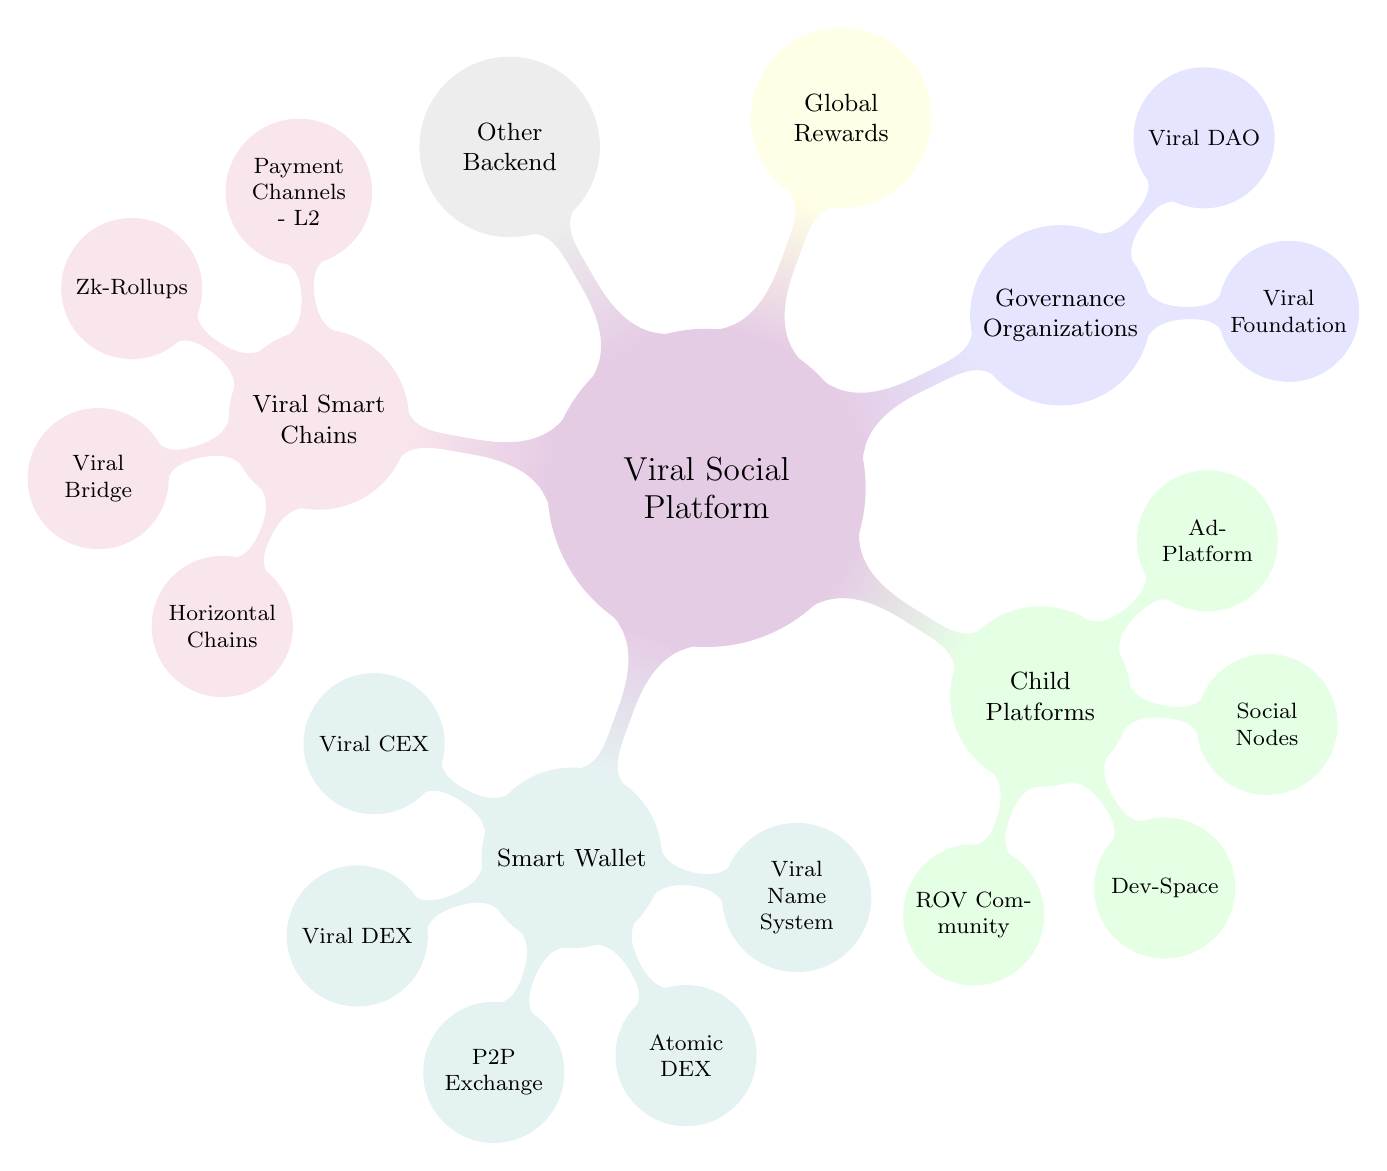
\begin{tikzpicture}
      [mindmap,
      grow cyclic,
      every node/.style=concept,
      concept color=violet!20,
      level 1/.append style={sibling angle=360/6},
      level 2/.append style={sibling angle=50},
      ]
      \node [root concept] {Viral Social Platform}
        child [concept color=purple!10, rotate=-40]{
          node    {Viral Smart Chains}
          child { node    {Payment Channels - L2} }
          child { node    {Zk-Rollups} }
          child { node    {Viral Bridge}}
          child { node    {Horizontal Chains} }
        }
        child [concept color=teal!10, rotate=-20]{
          node     {Smart Wallet}
          child { node    {Viral CEX} }
          child { node    {Viral DEX} }
          child { node    {P2P Exchange} }
          child { node    {Atomic DEX} }
          child { node    {Viral Name System} }
        }
        child [concept color=green!10, rotate=-2]{
          node  {Child Platforms}
          child { node {ROV Community} }
          child { node {Dev-Space} }
          child { node {Social Nodes} }
          child { node {Ad-Platform} }
        }
        child [concept color=blue!10, rotate=-4]{
          node  {Governance Organizations}
          child { node {Viral Foundation} }
          child { node {Viral DAO} }
        }
        child [concept color=yellow!10, rotate=-20]{
          node   {Global Rewards}%[clockwise from=45, level distance=8cm]
        }
        child [concept color=black!7, rotate=-30] {
          node {Other Backend}}
        ;  
        
        \end{tikzpicture}
\end{adjustbox}
\end{center}

\begin{enumerate}

\item \textbf{Viral App}: Decentralized Social Media Platform bridging Blockchain applications for limitless possibilities.

\item \textbf{Viral Smart Chains}: Horizontally Scalable EVM Smart Chain on Top of IOTA\textsc{\char13}s Tangle.

\begin{enumerate}

	\item \textbf{Payment Channels (L2)}: State Channels to move value off-chain for lightning fast micro-transactions.

	\item \textbf{Zk-Rollups (L2)}: Batching Multiple Off-chain NFT Standard Tokens (ERC721) to On-Chain,
	\item \textbf{Viral Bridge}: Interopability of various major cryotocurrencies by wrapping tokens decentralized such as Bitcoin, Ethereum,etc into Viral Smart Chains.
	\item \textbf{Horizontal Chains}: Additional of New Chains anchored to IOTA Tangle that communicates between multiple Viral Smart Chains for unlimited scaling

\end{enumerate}

\item \textbf{Smart Wallet}: Viral\textsc{\char13}s App\textsc{\char13}s built in Non-Custodial Viral Smart Chain compatible hot wallet that allows user to send and hold tokens, mint NFTs and receive rewards.

\begin{enumerate}

\item \textbf{Viral CEX-Centralized Exchange}: Trustless Non-Custodial Exchange for Fiat-Crypto trading
\item \textbf{Viral DEX-Decentralized Exchange}: Automated Market Making Protocol for exchanging Viral tokens
\item \textbf{P2P Exchange}: Trustsless anonymous exchange leveraging Peer-to-Peer protocol
\item \textbf{Viral Name System}: Decentralized blockchain based username protocol for transfers instead of cryptographic public address.

\end{enumerate}

\item \textbf{Child Platforms}: Independent platforms anchored to the viral network for effective improvement of protocols

\begin{enumerate}

\item \textbf{Dev-Space}: Application for Developers to decide on reward allocation for improving Viral-Beta
\item \textbf{ROV Community}: Curator Platform to vote and remove reported content on Viral-Alpha
\item \textbf{Ad Platform}: Decentralized Ad platform connecting Influencers,businesses and users for trustless engagement-proof ads.

\end{enumerate}

\item \textbf{Global Rewards}: To incentivize all users, miners, developers using smart contracts for their content, validation of transactions, and continuous development through unbiased pointing strategy that offers more rewards to bigger contributors.


\item \textbf{Other Backend}: For contingencies which will be later decentralized in the further phases of the development roadmap

	

\end{enumerate}

	\subsection{Development Tech Stack}

	\begin{enumerate}

	\item \hyperlink{https://ipfs.io}{IPFS}: IPFS stands for Interplanetary File System is a peer-to-peer distributed file system that is used for maintaining and distributing files across our Viral IPFS Private network.

	\item \hyperlink{https://gun.eco/}{GunDB}: GunDB is a fully decentralized graph database to store information from user to user meaning that your changes are not affected by any centralized server.

	\item \hyperlink{https://webrtc.org/}{WebRTC}: WebRTC stands for Web Real-Time Communication, an open-source project built primarily for peer-to-peer real-time connections.

	\item \hyperlink{https://www.javascript.com/}{Javascript}: JavaScript is a text-based programming language used both on the client-side and server-side that allows you to make web pages interactive.

	\item \hyperlink{https://nodejs.org/}{NodeJS}: Node.js is an open-source, cross-platform, back-end JavaScript runtime environment that runs on the V8 engine and executes JavaScript code outside a web browser.

	\item \hyperlink{https://reactjs.org/}{ReactJS}: React is a free and open-source front-end JavaScript library for building user interfaces based on UI components.

	\item \hyperlink{https://docs.soliditylang.org/}{Solidity}:Solidity is an object-oriented, high-level language for implementing smart contracts, mostly used for executing code in Ethereum Virtual Machine

	\item \hyperlink{https://wiki.iota.org/smart-contracts/overview}{IOTA Smart Contract Protocol}: The IOTA ecosystem allows to spin up a smart contract blockchain and anchor it to the IOTA tangle
	
	\end{enumerate}


\section{How Whitepaper Structured}
For an efficient understanding, we have seperated the Viral Architecture/Ecosystem\textsc{\char13}s major sectors.\\

\begin{itemize}
\item Social Media and User Experience (Page 1-10)
\item Blockchain, Token Ecosystem and Layer 2 (Page 10-15)
\item Smart Wallet (Page 15-20)
\item Child Platforms (Page 20-25)
\item Revenue and Incentives (Page 25-30)
\item Viral DAO  and Governance
\end{itemize}

\section{Social media and User Experience}
Viral is a multi-media sharing decentralized social network that brings meta-experience with friends, family and other people to communicate, share posts and send messages across the globe with absolute privacy. Viral sets Non-Fungible-Tokens (NFT) as a standard for every post that shared in the network which intends to bring interactive social experience and utility use cases of blockchain environment.\\

\notte{To bring NFT as a standard for a social media post doesn\textsc{\char13}t essentially implies it ought to be sold for tokens, rather it conveys that each post in Viral is a unique piece of data in the blockchain that gives the power of ownership of the user which if needed can be opted to transfer in exchange for tokens inside the Viral Platform.\texttt{notte}.}

\begin{lstlisting}[language=Solidity, caption={NFT Snippet for Enable/Disable Open Sale}]

pragma solidity ^0.8.10;

contract HelloWorld {

    string public greet = "Hello World!";
    
}
\end{lstlisting}

\subsection{Types of Post}
\hyperlink{https://sample.com}{ELI5 Explanatory Video - Viral NFTs}\\

Please read \hyperlink{App Brouchure}{https://sampel.com/} to have a visual experience of the Viral Social Network\\

\textit{Image for all Post Types in a Visualized Manner}

\subsubsection{Shots}

Shots are \textbf{10 sec motion pictures} with added loop transitions to bring life to photos. Pictures can be shared as shots, an exciting looped motion picture.\\

People can share their
\begin{enumerate}
\item Personal Sneak-Peek, Moments and Events
\item Exclusive Photoshoots, commercials, to your fans
\item Turn photos into lively shots by adding shot animations through Viral
\end{enumerate}

\subsubsection{Thoughts}
Thoughts are \textbf{text-based sharing} for micro-blogging. Attach photos, long/short videos, documents, etc. There is no limit on words or media. People can share other users thoughts to their followers using re-Thought feature.

\subsubsection{Drops}
Drops are \textbf{20 second disappearing stories} shared to followers which auto-disappears once seen. It features AR filters, texts, shot elements, links, music, transitions and, much more. Every Drops will be purged in 30 days\\

\notte{Drops will not be minted as unique NFT due to it\textsc{\char13}s nature of disappearing media\texttt{notte}.}

\subsubsection{Interactive Videos}
IVs are short 30sec full-screen\textbf{narration based videos}. It is based on\textbf{gamification of videos} to interact within the videos.

\subsubsection{NFT Utilities}
Minting (Creating) an NFT in Viral is\textbf{as easy as creating a social media post}. Viral provides multiple NFT utilities for users to mint, buy, sell with an easy user experience.

Viral will take a\textbf{1.5\% commission} selling NFTs which will be reverted to the reward pool

\subsubsection{Tunes}

Artists can\textbf{sell their music albums}, singles as NFT for the fans/people to buy and own it

\begin{lstlisting}[language=Solidity, caption={NFT Snippet To Sell Multiple Copies}]

pragma solidity ^0.8.10;

contract HelloWorld {

    string public greet = "Hello World!";
    
}
\end{lstlisting}

\subsubsection{Sketch}
\textbf{Digital arts}, paintings, sketches can be sold through NFTs

\begin{lstlisting}[language=Solidity,label={single-asset}, caption={NFT Snippet to sell single asset}]

pragma solidity ^0.8.10;

contract HelloWorld {

    string public greet = "Hello World!";
    
}
\end{lstlisting}

\subsubsection{Originals}
\textbf{Physical assets} can be sold through Viral\textsc{\char13}s Original NFTs where people can buy and flex

\begin{lstlisting}[language=Solidity, caption={NFT Snippet to provide extra information such as Name, Address, Mobile Number, before transferring coins with end to end encryption between seller}]

pragma solidity ^0.8.10;

contract HelloWorld {

    string public greet = "Hello World!";
    
}
\end{lstlisting}

\subsubsection{Tickets}
\textbf{Exclusive passes} for events, ownership of clubs, a digital ticket for everything can be sold as NFT. See Listing \ref{single-asset}

\subsubsection{Filters}
Filters can be sold, and owned by user\textsc{\char13}s thereby get rewards for it

\begin{lstlisting}[language=Solidity, caption={NFT Snippet to distribute shares Just like company share where if 100 NFTs is sold, the person who holds 50 NFT will hold 50\% of the company}]

pragma solidity ^0.8.10;

contract HelloWorld {

    string public greet = "Hello World!";
    
}
\end{lstlisting}

Please read \hyperlink{App Brouchure}{https://sampel.com/} to have a visual experience of the Viral Social Network

\subsection{Avatars}

Personalized Avatars are generated free for every viral user using a selfie. Users can edit their avatar skin, outfit, hair, etc. These avatars will be shown in their public profile where other users can see them 3D View.\\

\textit{Image}\\

These avatars are brought into Viral to integrate metaverse and to provide an \textbf{interactive experience}\\

\hyperlink{https://sample.com}{Avatar Demo-Video}\\

\begin{lstlisting}[language=Solidity]

// ReadyPlayerMe Integration Examples

1. ReadyPlayerMe WebView- How creating Avatars work using Partner API
2. Downloading Asset- GLB File using Event Listener
3. Mapping skeletons and face
4. Animating and storing the file as a 3D Viewer File inside the application using IPFS Public/Clusters
5. How Animations will work

\end{lstlisting}

\subsubsection{Meta-Chat}

Meta-Chat is a feature to \textbf{show your facial reactions} in real-time when you chat with your friend. Viral captures your face reactions and transfer it to your avatar which the mutual friend can see on \textbf{top of his/her chat page}.

\textit{Image}\\

This gives you a \textbf{virtual experience} of videocalls through avatars and text chat.

\hyperlink{https://sample.com}{Meta-Chat Demo}\\

\textbf{SDKs and APIs Used} : List the APIs\\

\textit{Formula\\
Flowcharts}

\subsubsection{Live and Rooms}

Decentralized \textbf{Live Video Events and Audio Rooms using Avatars} (or) Normal Cams. Celebrities can host live events with their fans using their avatars\\

\textit{Image}\\
\hyperlink{https://sample.com}{Live-Events Demo}\\

\textbf{SDKs and APIs Used} : List the APIs\\

\textit{Formula\\
Flowcharts}

\subsection{Engagements}

\textbf{Like, Comment, Share, Tip}\\

Users can like, comment, share, reThought, and also tip Tokens to their favorite posts and influencers. The number of likes will influence the recommendations list of other users.\\

Additionally a hidden engagement dislike will be added to every post but won\textsc{\char13}t be visible to the users/nor owners, which is exclusively utilized for interest-based algorithm to filter out disliked content\\

\textit{Algorithm/Mathematical formula for recommendation engine}\\

\textbf{Tip}\\

The tipping feature in Viral engagements tip/support user\textsc{\char13}s favourite influencers\textsc{\char13} contents. It works as a donation/reward where all the tips will be directly sent to the receivers wallet. Users can send tokens of their own choice to reward other users content on the platform.

Viral will charge commisions on Tips and deposits it to the reward pool. These commissions are calculated in such a way where the percentage varies depending on the end face value.\\

The tipping amount will be round of to tens and will leave the commision on both seperated amounts.\\

$Formula$\\

The Charges are\\


(Ending with 1,2)\$ tips     - 22\%      i.e., 11, 62, 761, 952\\
(Ending with 3,4,5)\$ tips   - 19\%      i.e., 23, 64, 765, 953\\
(Ending with 6,7,8,9)\$ tips - 17\%      i.e., 16, 48, 27,  79\\
(Ending with 0)\$ tips       - 12\%      i.e., 10, 60, 720, 1000\\


For example: If a user is tips worth 57\$ then the commissions charged will be:\\

For the first     50\$ - 12\%\\
And the remaining 7\$  - 17\%\\
\begin{figure}[H]
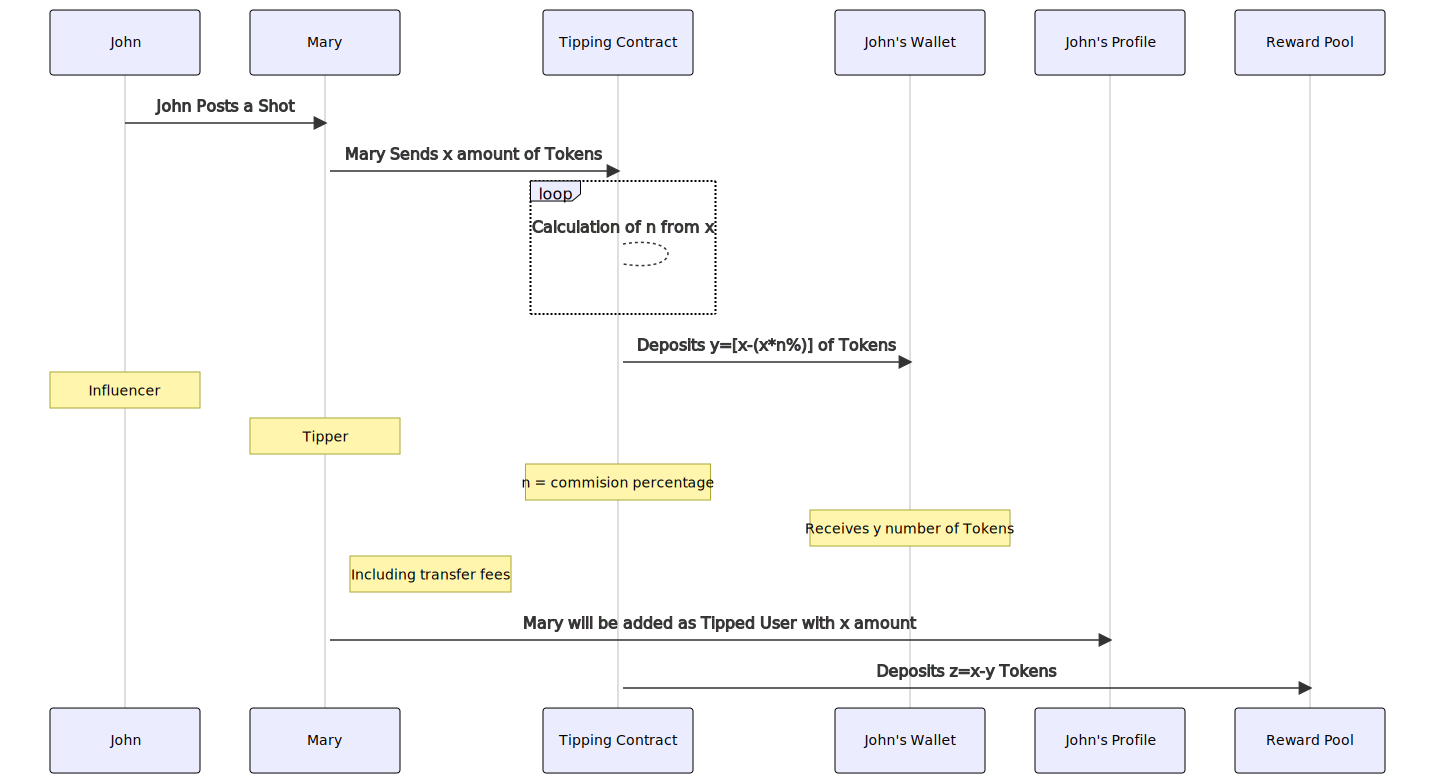
\includegraphics[width=\textwidth]{tips}\\
\caption{Tips Flowchart}
\end{figure}

\begin{comment}%mermaid

sequenceDiagram

    participant John
    participant Mary
    participant Tipping Contract
    participant John's Wallet
    participant John's Profile
    participant Reward Pool
    

    John->>+Mary:John Posts a Shot
    Mary->>+Tipping Contract:Mary Sends x amount of Tokens
    loop 
    Tipping Contract-->Tipping Contract:Calculation of n from x
    end
    Tipping Contract->>+John's Wallet:Deposits y=[x-(x*n%)] of Tokens
    Note over John: Influencer
    Note over Mary: Tipper
    Note over Tipping Contract: n = commision percentage
    Note over John's Wallet: Receives y number of Tokens
    Note right of Mary: Including transfer fees
    Mary->>+John's Profile: Mary will be added as Tipped User with x amount
    Tipping Contract->>+Reward Pool: Deposits z=x-y Tokens

\end{comment}


\begin{lstlisting}[language=Solidity, caption={Tipping Solidity Snippet}]

pragma solidity ^0.8.10;

contract HelloWorld {

    string public greet = "Hello World!";
    
}

\end{lstlisting}

\subsection{Other Features}

\subsubsection{Privacy Groups}

Privacy Groups is a unique feature in Viral to create unlimited friend\textsc{\char13}s groups list to ensure maximum privacy for users to post and share to particular groups of users i.e., Family, Friends, Close Friends, Besties, etc. This feature can empower complete privacy over viewers for certain posts.\\

\begin{figure}[H]
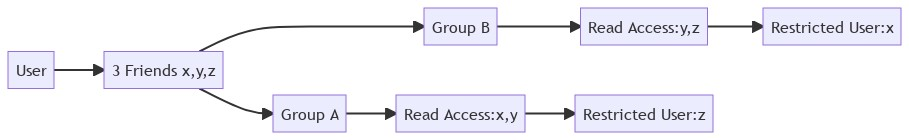
\includegraphics[width=\textwidth]{privacygroups}\\
\caption{Privacy Groups}
\end{figure}

\begin{comment}%mermaid
flowchart LR
    A[User]-->0
    0[3 Friends x,y,z]-->B[Group A]
    0--->C[Group B]
    B-->D[Read Access:x,y]
    C-->E[Read Access:y,z]
    D-->F[Restricted User:z]
    E-->G[Restricted User:x]
\end{comment}

\begin{lstlisting}[language=Solidity, caption={GunDB Privacy Group Snippet}]

pragma solidity ^0.8.10;

contract HelloWorld {

    string public greet = "Hello World!";
    
}
\end{lstlisting}

\subsubsection{Audio Emoji}

This is a short feature where all the emojis in Viral if touched will give a \textbf{short sound of the emoji}. This will be accessible on chats and comments section of a post.\\

\subsubsection{Interest Based Recommendation}

To make the viral platform more user-friendly interest-based recommendations are utilized. We have numerous ways to fetch interest from a user \textbf{without collecting data on a centralized server}, a few of them are\\

\begin{itemize}[leftmargin=+0.2in]
\item Like and Dislike
\item Hashtag Follows
\item Search-Based Interests
\item Based on Activity
\item Shares with other friends
\item Following interests
\item Based on Comments
\end{itemize}

All the user interests will be \textbf{stored locally} on the device to ensure \textbf{maximum security} and will be taken to show recommendations.\\

$Flow chart$

\subsection{User Security and Privacy}

$Abstract$\\

This is classified into\\
\begin{enumerate}[leftmargin=+0.2in]
\item Media Storage
\item Chats or Private Messages
\item Interests of User
\item Chat backups
\end{enumerate}

\textbf{1. Media Storage}\\

All Media uploaded to Viral is End-to-end Encrypted where all the files are encrypted using Symmetric AES-256 Encryption Standard on the device and gets uploaded to Trustless IPFS Public Nodes and Trusted IPFS Cluster Nodes. Thus promising the security of media.\\

\textbf{Encryption}\\

$Detailed Explanation$\\


\begin{figure}[H]
\begin{center}
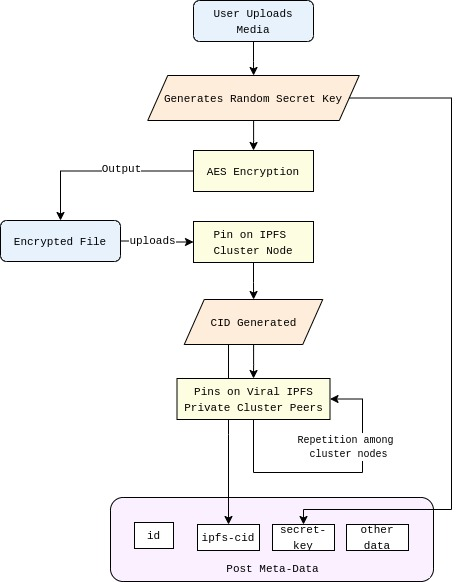
\includegraphics[width=6cm]{encryption}
\caption{Encryption of Media in Viral}
\end{center}
\end{figure}

\begin{comment}
flowchart TB

  subgraph Offline Process
  A([<font size=5>User Uploads Media])--<font size=5>1-->B([<font size=5>Generates secret-key])
  B--<font size=5>2-->C[<font size=5>Encrypted Locally]
  end
  subgraph Post-MetaData
  subgraph static
  L[<font size=5>id]
  R[<font size=5>IPFS-URI]
  U[<font size=5>secret-key]
  end
  subgraph dynamic
  P[<font size=5>other-data]
  end
  end
  subgraph IPFS
  D[/<font size=5>File Upload to IPFS Public/]--<font size=5>5-->G([<font size=5>Receives IPFS-URI])
  G--<font size=5>6-->E[<font size=5>Pins IPFS-URI to Viral's IPFS Cluster]
  E--<font size=5>7-->F[<font size=5>Cluster repetition = min:8 max:15]
  end
  B--<font size=5>secret-key-->U
  IPFS--<font size=5>8------>K2[/<font size=5>Add IPFS-URI/]-->R
  C--<font size=5>3-->K1[<font size=5>Encrypted File]--<font size=5>4-->D
  Post-MetaData--<font size=5>9-->K3([<font size=5>Content is Stored])

\end{comment}



\textbf{Decryption}\\

Private Account Media Decryption\\

$Detailed Explanation$\\

\begin{figure}[H]
\begin{center}
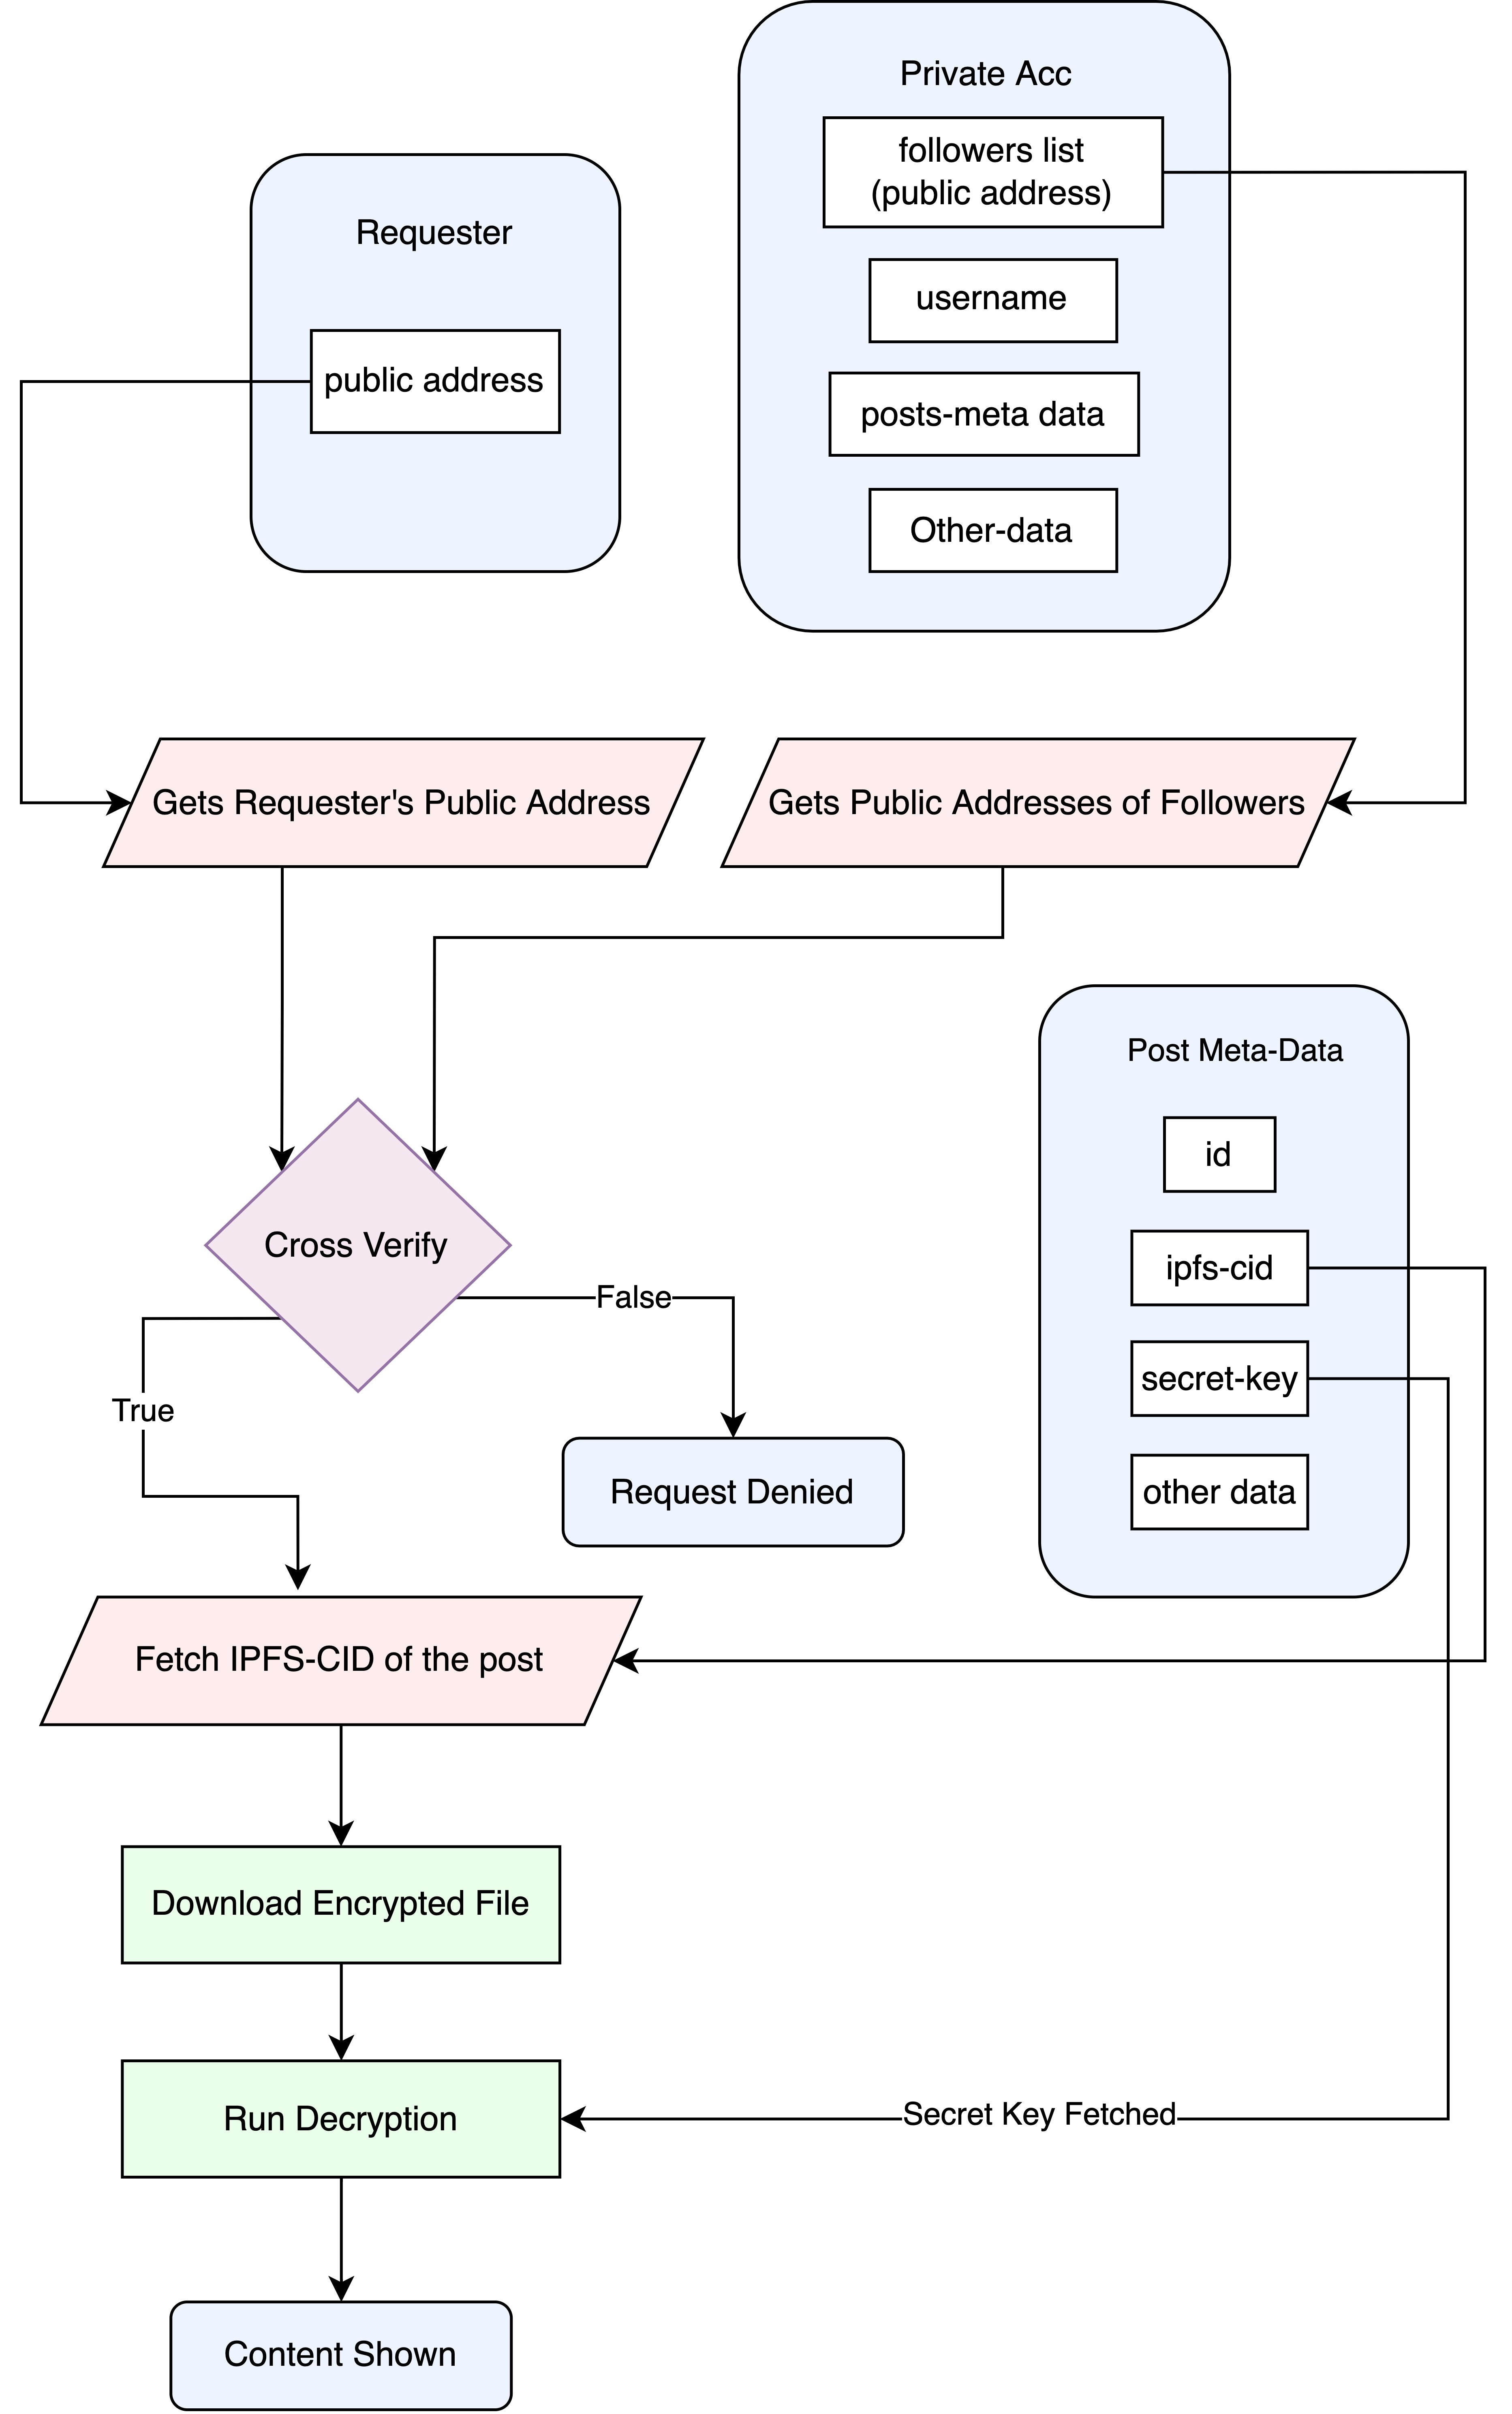
\includegraphics[width=\textwidth]{decryption-private}
\caption{Decryption Media of Private account in Viral}
\end{center}
\end{figure}

\begin{comment}

flowchart LR
subgraph Private-Account-Media-Decryption
  A0[User A request to view User B content]
  subgraph Follower Verification
  A0--1-->A1
  A1[Gets User A Public Address]
  A2[Gets User B Followers' Public Addresses]
  A3[Cross verify]
  A4[Content-Access Denied]
  A1--2-->A3
  A3--No-->A4
  A2-->A3
  end
  subgraph IPFS-Download-Process
  C1[URI is Fetched]
  C2[Download's Encrypted File]
  C1--5-->C2
  end
  A3--3-->K1[Sucessful]--4-->IPFS-Download-Process
  subgraph User-B-Private-Account
  B1[username]
  B2[Followers-Public-Addresses]
  B3[All Posts Meta-Data]
  B4[Other Data]
  end
  B2-->A2
  subgraph User-B-Post-MetaData
  subgraph static
  id
  IPFS-URI
  secret-key
  end
  subgraph dynamic
  other-data
  end
  end
  IPFS-URI-->C1
  B3-->User-B-Post-MetaData
  subgraph Decryption-of-encrypted-file
  D1[secret-key is Fetched]
  D2[Decrypt's the File]
  D1--7-->D2
  end 
  secret-key-->D1
  C2--6-->Decryption-of-encrypted-file
  Z[Content is shown]
  D2--8-->Z
end

\end{comment}


Public Account Media Decryption\\

$Detailed Explanation$\\

\begin{figure}[H]
\begin{center}
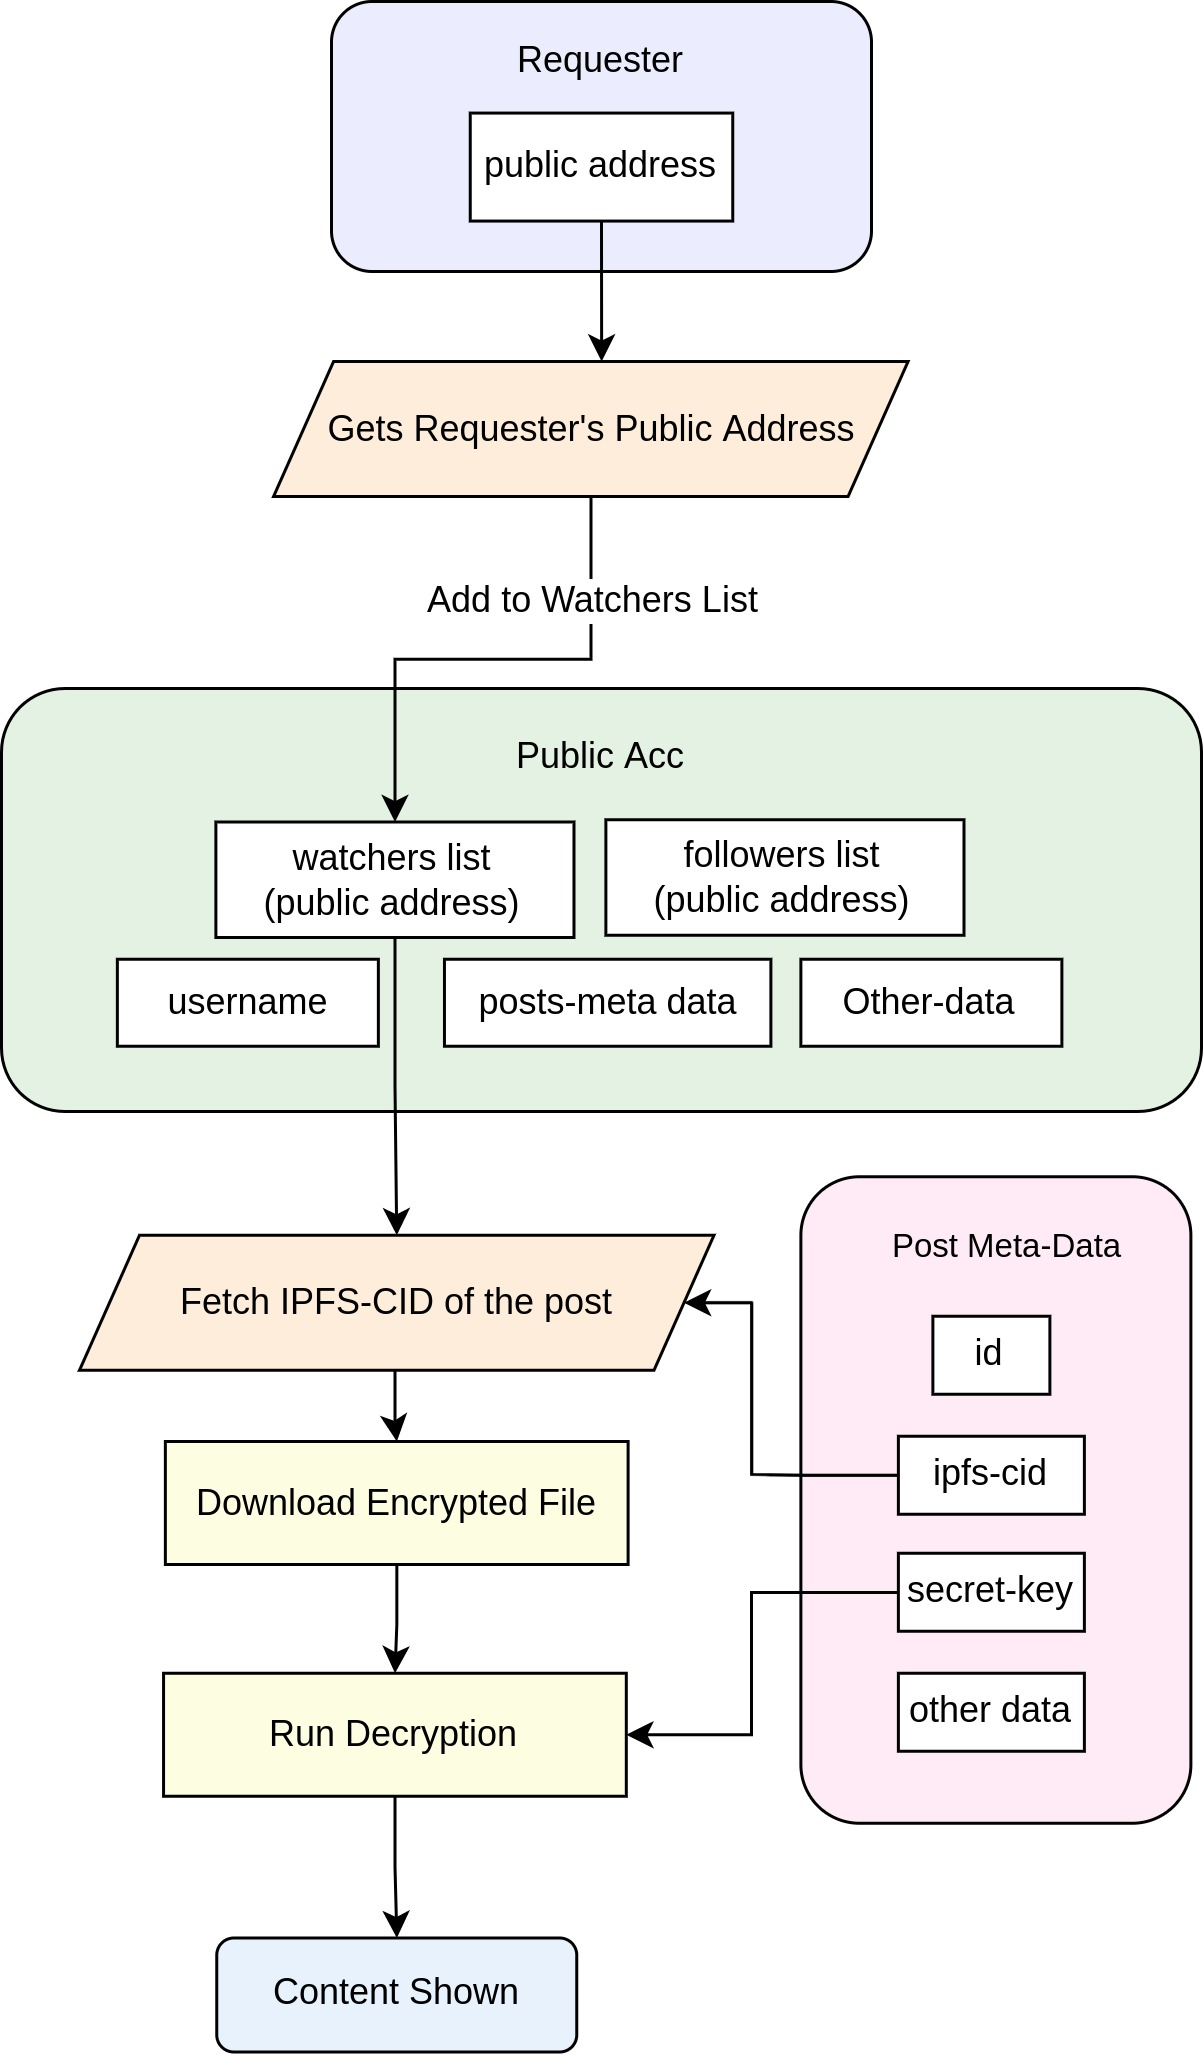
\includegraphics[width=6cm]{decryption-public}
\caption{Decryption Media of Public account in Viral}
\end{center}
\end{figure}

\begin{comment}
flowchart LR
subgraph Public-Account-Media-Decryption
  A0[User request to view a Public Account]
  subgraph User Request
  A0--1-->A1
  A1[Gets User's Public Address]
  end
  subgraph Public-Account
  B1[username]
  B2[Watchers-Public-Addresses]
  B3[All Posts Meta-Data]
  B4[Other Data]
  end
  A1--2-->K1[Add to Watchers List]--3-->B2
    subgraph IPFS
  C1[URI is Fetched]
  C2[Download's Encrypted File]
  C1--5-->C2
  end
  subgraph Decryption-of-encrypted-file
  D1[secret-key is Fetched]
  D2[Decrypt's the File]
  D1--7-->D2
  end 
  subgraph User-Post-MetaData
  subgraph static
  id
  IPFS-URI
  secret-key
  end
  subgraph dynamic
  other-data
  end
  end
  IPFS-URI--->C1
  secret-key--->D1
  B3--->User-Post-MetaData
  B2--4-->IPFS
  C2--6-->Decryption-of-encrypted-file
  Z[Content is shown]
  D2--8-->Z
end
\end{comment}


\textbf{2. Chats and Private Messages}\\

For Chat-based encryption, Viral uses \textbf{public and private key} encryption method. There are no centralized cloud-based servers involved in storing messages which can potentially trigger breaches. Every single message is encrypted and can be only decrypted by the receiver.\\

Public-Private key encryption more secure than a single shared key which is utilized in multiple chat platforms.\\

$Visual Representation$\\

Alice writes and Hello and to Bob – Bob Receives an encrypted message - Bob decrypts using his private key – Bob Sees and Hello from Alice

\hyperlink{https://sample.com}{GunDB Explanatory Video}\\

\textbf{3. Interests of User}\\

Users\textsc{\char13} interests will be \textbf{saved locally} on their devices ensuring full privacy of personal data.\\

\textbf{4. Chat Backup}\\

Since Viral is a \textbf{Offline-First Chat} messages will not be stored in cloud. To Backup messages Viral will offer \textbf{cloud options} such as Google Drive/Dropbox where you can securely encrypt and save your \textbf{backup}. While Migrating to another mobile we will be providing a feature to transfer existing messages/interest to your new device.\\

\textbf{Phase 2 Development}\\

We will be focussing on Quantum Resilience of all media encryption used in Viral while commencing the Phase 2 of Development Roadmap\\

\subsection{TOR/VPN Anonymity}

Viral will be a safe haven for anonymity, privacy, and security in eliminating the tracing of users\textsc{\char13} identities by exploiters . Users can benefit from TOR and VPN Routing Features built in our Decentralized application to hide their IP address and go fully anonymous.\\

TOR routes you through several additional nodes while encrypted, no one can trace it back to you. VPN will redirect your internet traffic through a secure tunnel, hiding your IP address and encrypting your data in the process.\\

\textbf{Content Delivery}\\

Visualization with changes to minting as NFT\\

AES – 256 Encryption Snippet\\

\textbf{IPFS Cluster}\\

Visualization of Repetition\\

Addition of Nodes – Trusted Way\\

Phase 2 – Trust less Way (IPFS-VM)\\

\section{Blockchain, Token Ecosystem and Layer 2}

\subsection{Viral Smart Chain – Short Intro}

Viral Smart Chains, is a network of horizontally scalable EVM Chains on top of IOTA Tangle used for Viral Social network with fully deployed defi ecosystem with Off-Chain solutions. Viral Smart Chains aim to provide an easy understandable one-platform for all the non-crypto users who are subjected to higher gas fees, congestion in network, volatility and scattered defi solutions.\\

\subsection{IOTA Smart Contract Protocol}

IOTA provides an Off-Chain Smart Contract Solution for developers to create multiple-chains on Top of IOTA\textsc{\char13}s immutable Tangle. Since Ethereum transactions are processed On-chain by every single node on its network, it faces additional congestion, slow transaction time and subject to higher miner fees. IOTA\textsc{\char13}s off-chain smart contract solution makes use of blockchains anchored to the Tangle where the smart contracts are ran and achieved consensus with small set of committee nodes. This achieves a high scalable throughput and immutable records since the states of smart contracts such as Account Balances, Input Conditions and Consequences over time are updated on IOTA\textsc{\char13}s Tangle.\\

There are several components to understand more about IOTA\textsc{\char13}s Smart Contracts Protocol. It gives us multi-chain functionality to run smart contracts from different chains which allows a horizontal scaling of blockchains without a need for plasma or side chains.\\

\textbf{Consensus and Validators}\\

IOTA\textsc{\char13}s Smart Contract Chain uses a Byzantine Fault Tolerant \(BFT\) Algorithm, which guarantees consistency and byzantine fault tolerance if less than $1/3$ of nodes are malicious. So the verification process runs on Nodes within a chain committee. With a Proof-of-Stake Consensus each Viral chain will be run by a network of validator nodes, which run a consensus on the chain state updates. The validators of the chain \(Nodes\) form a committee, a bound together closed set of nodes. The committee of the chain can allow new validators and validator nodes to be added or replaced. This also makes the chain itself agnostic to its validators \(the committee\).\\

Viral Smart Chains leverages IOTA Tangle\textsc{\char13}s properties of scalability, high throughput, feeless transactions and immutable records. Only when a supermajority of the validators (the quorum) of a chain reaches consensus, the results get added to the chain where a new state update can be signed, which unlocks the AliasOutput for the chain and produces the next state UTXO which is stored on the Tangle as an immutable record. In summary, the chain\textsc{\char13}s state (data) will be stored on Tangle as an immutable record.The amount of the validators to reach a consensus is configurable for each chain. The committee itself can also be variable in size - from a few nodes up to hundreds of nodes, and each node can be part of many different committees.

\begin{itemize}[leftmargin=+0.2in]
\item \textbf{Validators} – Each Single Node running the Chain
\item \textbf{Committee} – The Group of Nodes running a chain
\item \textbf{Quorum} – Number of Nodes to be in consensus to validate a transaction
\end{itemize}

To know more about IOTA\textsc{\char13}s Smart Contracts : \hyperlink{https://files.iota.org/papers/ISC_WP_Nov_10_2021.pdf}{Whitepaper}, \hyperlink{https://wiki.iota.org/smart-contracts/overview}{Documentation}, \hyperlink{https://blog.iota.org/iota-smart-contracts-beta-release/}{Blogs}\\

\subsection{Viral Smart Chains}

Viral Smart Chains are a family of separate chains anchored to the IOTA\textsc{\char13}s Tangle where each chain can communicate with each other via intermediary L1 Value Tangle.\\

\textbf{Viral\textsc{\char13}s Approach}\\

A Single chain will seem complex for setting different fees for different actions on the blockchain i.e Smart Contract Calls/Deployment, Sending Tokens to other Address, etc. Viral\textsc{\char13}s approach is to bring multiple chains categorized by its purpose to serve the Viral Application with fee structure thereby also creating separate chains to provide zero network fees for minting NFTs on Viral App (ERC721 and ERC1155) while rewarding the validators of all Viral chains (including zero fee chains) from the miner pool (total collected fees of all chains) based on validator\textsc{\char13}s total validated transactions for the day through an automated smart contract.\\

\textbf{Validators}\\

Viral Chains will work on Proof-of-stake consensus where validators (miners) are required to stake their Viral Coins in order to participate in the network for validating transactions. The mining power in proof-of stake depends on the amount of coins a validator is staking. Participants who stake more Viral Coins will be most likely to be chosen to add more blocks. When a transaction is validated and attain consensus by the quorum of validators (Read IOTA Protocol), the state of the transaction/smart contract will be recorded in the Value Tangle\textsc{\char13}s UTXO Ledger which makes it immutable. The Transaction will be secured by the validators inside the Viral chain and also the L1 UTXO Ledger.\\

\textbf{Fees}\\

Viral Smart Chain is built primarily to ease the need for gas-based transaction fees like other smart contract blockchains. Transaction fees are only leaved as a fixed percentage as andquot;transfer feeandquot; in Viral Smart Chains for Sending, receiving tokens between accounts and smart contracts.\\

Transfer fees are fixed at 0.05\% of transfer value of the tokens paid in Viral native coin. The minimum fee is capped at \$0.0005 of the fiat value of Viral Coin which is determined using price oracles.\\

$Visualization$\\

Native Token : Bob wants to transfer 100VRL to John : Fee leaved will be 0.05 VRL\\

Other Tokens : If 1 vMATIc = 0.1 VRL\\

Mike wants to transfer 6000 vMATIC to Mia : Fee leaved will be 0.30075 VRL (approx. 3.0075 MATIC) including Swap and Transfer Fee\\

\textbf{NFT Chains}\\

Currently on popular smart contract blockchains such as Ethereum, Polygon the amount of gas required for a transaction is determined by the demand for the transaction to be included, regardless of what type of transaction it is where it is dynamically adjusted based on number of user\textsc{\char13}s interacting with the network at the time.\\

This brings us to an effect that a single blockchain cannot set certain fees or eliminate gas fees for a particular type or category of a transaction regardless of it\textsc{\char13}s nature i.e, smart contract, account transfer. Multiple parallel state blockchains can solve this issue by altering few blockchains as permissioned for a certain use cases and can make it feeless without hindering the other fee-based chains.\\

Viral\textsc{\char13}s aim to democratize NFT to the masses and bring massive NFT Adoption we will be running separate zero-fee chains for deploying ERC721 and ERC1155 Token directly from the Viral Application. The Validators for the chain will be open to join the network where they\textsc{\char13}ll be rewarded from the miner pool (total fee collected) based on the total transactions they validate in a day.\\

\textbf{Family of Chains}\\

\begin{comment}%mermaid chainfamily
graph TD
    A[Genesis Chain]
    B[General Chains]
    B-->J[Description]
    C[De-Fi Chains]
    D[DEX Chain]
    E[Fungible Contract Chains]
    F[Non-Fungible Contract Chains]
    G[Viral NFT Chains]
    H[Marketplace Chains]
    I[Other DApp Chain]
    A-.-B
    A-.-C-.-D & E & F & G & H & I
\end{comment}

\begin{itemize}[leftmargin=+0.2in]
\item \textbf{Genesis Chain} : Initialization of First Chain with Viral Coin and Stable Coin Deployment with Smart Contracts that defines governance, fees, etc\\

\item \textbf{General Chains} : For Every n number of active Viral Wallet users a new general chain is deployed. These chains are used to store user funds and create new accounts on the blockchains. So Users can do intra and inter chain transactions with high throughput and flexible scaling.\\
\end{itemize}
\textbf{De-Fi Chains}\\
Smart Contract Deployment Chains specifically for categorized DApps\\
\begin{itemize}[leftmargin=+0.2in]

\item \textbf{DEX Chain} : Running smart contracts for Viral Wallet\textsc{\char13}s Decentralized Exchange

\item \textbf{ERC20 Chain} : To Deploy new ERC20 Tokens that can be transacted between chains and accounts

\item \textbf{Viral NFT Chain} : Feeless Viral ran Smart Contract Chain specifically to deploy user\textsc{\char13}s NFTs on-chain

\item \textbf{ERC721/115 Chain} : To deploy new Non-Fungible Tokens for other platforms outside the Viral Application

\item \textbf{Marketplace Chain} : To create smart contract based marketplaces for NFTs and much more

\item \textbf{Other Chains} : For creating Dapps for lending, asset tokenization, yield farming, tools and infrastructure, etc
\end{itemize}

Development

\begin{lstlisting}

      _Root_

      - _Initialization of the chain_
      - _Deployment of new contracts_
      - _Registary of contracts_
      - _Chain ownership management and Access control list_
      - _Fee management_

      _Accounts_

      - _On Chain ledger accounts_
      - _Securely moving tokens between accounts_
      - _Ensuring consistency of the on-chain ledger_

      _Eventlog_

      - _Keeping timestamp immutable log of On-Chain events_

      _Blob_

      - _Keeping registry of Binary objects of arbitrary sizew_

      _Configuration of Committee and quorum_

      _Wasp Nodes_

      _EVM Plugins_

      _Configuring Fees_

      _Smart Contract Deployments_

      _State Updates on Tangle_

      _Multi-Chain Integration_

      _Core-Contracts_

\end{lstlisting}

\subsection{Token Ecosystem}

\subsubsection{Viral Coin - Native Token}

Viral Coin is the native currency, a digital coin that does all the operations inside the Viral Smart Chains. It is used to store value, send and receive funds within the Multi-Chain Viral Blockchains. Viral Coin is used for paying fees inside the network, staking, governance, rewards and much more.\\

\subsubsection{Viral Stable Coin}

Viral Stable Coin is a sub-native token, an algorithmic stable coin pegged to the US Dollar that is widely used in the Viral Application for sending and receiving tokens across users wallets. Due to constant volatility of the crypto market there is a barrier for the common people and businesses to get into cryptocurrencies. As Viral\textsc{\char13}s aim to become the one-stop crypto solution for the masses we are providing a way for the user\textsc{\char13}s to automatically transact in Stable Coin without any complex need for swapping their current tokens. In Short, when an user transact in Viral Coin, he can opt to send the receiver viral stable coins to avoid depreciation of the asset while transacting.\\

As far as we know there are several stable coins are in the market 1.Fiat-Peg Centralized, 2.Crypto Collateral 3. Algorithmic. In our case we can take 3 coins 1. USDC 2. DAI 3. AMPL. USDC maintains the peg but holds the funds on its reserves centralized which comes with its demerits. DAI aims to maintain the peg using collateral of several crypto coins, in which USDC hold the reserve of more than 50\% of the DAI\textsc{\char13}s crypto backing, which also makes DAI a centralized cryptocurrency. AMPL is an algorithmic stable coin which maintains it\textsc{\char13}s peg by contracting and expanding it\textsc{\char13}s supply of tokens to achieve stability, this achieves true decentralization but fails to operate swiftly for sudden price movements due to it\textsc{\char13}s rebase function ran in a stipulated time and also rebases in a slow, long way which takes upto a week after a sudden price movement. This is where most crypto projects fail to provide a decentralized stable currency for the masses.\\

Terra blockchain is the most successful running algorithmic stable coin which maintain its stability by changing the stable coin\textsc{\char13}s supply by burning and minting it\textsc{\char13}s native token LUNA. In better words, when Terra (Stable Coin) demand increases to more than \$1, Luna (Native token) will be burned and New Terra tokens will be minted, where increase in supply of tokens resolves the demand and maintains the peg of the stable coin and vice versa. Viral Stable Coin adopts the algorithmic stable coin algorithm used in many of Terra\textsc{\char13}s stable coins.\\

Viral Coin and Viral Stable Coin will be the two primary coins in the Viral Social Platform. The supply and demand of Stable Coin is always balanced by making Viral Coin as it\textsc{\char13}s variable counterweight that absorbs it\textsc{\char13}s volatility.\\

\textbf{1 VSC - \$1 (Expansion)} : When Viral Stable Coin trades at a price that is high relative to it\textsc{\char13}s \$1 peg i.e., \$1.15, the demand for VSC is higher than the circulating supply. To bring the peg back to \$1, the supply of VSC should be increased to balance the demand. During Expansion State trading bots will mint VSC by burning VRL, which has an effect of lowering Viral Stable Coin Price (by expanding the supply) and increases the Viral Coin price (by reducing it\textsc{\char13}s supply). The smart contracts will trade until the price peg of 1 VSC = \$1 is achieved.\\

$Formuka for Expansion$\\

\textbf{1 VSC - \$1 (Contraction)} : When Viral Stable Coin trades at a price that is low relative to it\textsc{\char13}s \$1 peg i.e., \$0.95, the demand for VSC is lower for the circulating supply. To bring the peg back to \$1, the supply of VSC should be decreased to balance the demand. During Contraction State trading bots will burn VSC and mints VRL, which has an effect of increasing Viral Stable Coin Price (by reducing it\textsc{\char13}s supply) and lowering the Viral Coin price (by expanding it\textsc{\char13}s supply). The smart contracts will trade until the price peg of 1 VSC = \$1 is achieved.\\

\textbf{Viral Stable Trading App}\\

High Frequency trading cannot be run using automated smart contracts to maintain price peg of Viral Stable Coin. Users can stake their Coins, run automated arbitrage trading and receive profits using the Viral Stable Trading Application a separate application to maintain the peg of Viral Stable Coin\\

Users will be able to stake both coins VRL and VSC proportionally to a smart contract in the mobile app which process all transactions of burning and minting VRL for VSC automatically without the need for user signature and receive profits from arbitrage opportunities by minting and burning the coins to balance the volatility. The Smart Contracts will add and subtract coins on each pools to maintain stability.\\

\subsubsection{Wrapped Tokens}

To acknowledge the tokenized economy Viral will bring popular cryptocurrencies such as Bitcoin, Ethereum, Dogecoin, etc into the Viral Smart Chains using wrapped token method. Since interoperability of blockchains are not possible (blockchains cannot talk to each other), centralized exchanges are used to exchange cryptocurrencies between each other using order books where the exchanges act as a custodian maintaining the user’s crypto holdings (E.g.: Bitcoin to Ethereum). To eliminate centralized processes, tokenization of other blockchain coins are introduced. Original Tokens will be reserved in it's native blockchain and a copy of the tokens, new wrapped tokens will be minted (created) on Viral Smart Chains. The wrapped tokens will be 1:1 pegged with the native cryptocurrency and can be used in various de-fi applications. Viral Smart Chain's approach is to develop several wrapped tokens of popular cryptocurrencies for its users to invest and exchange in a decentralized manner.\\

\textbf{Viral Decentralized Bridge}\\

Intro\\
Type of Viral Bridges\\
ERC20 Bridge\\
Abstract\\
List of Cryptocurrencies\\
Mechanisam\\
Flowcharts\\
UTXO Bridge\\
Abstract\\
List of Cryptocurrencies\\
Mechanism\\
Flowchart\\
Conclusion\\
Hence Users can invest in Bitcoin and other popular cryptocurrencies if they want to, without any hassles of other wallet applications or other blockchain wallets.

\subsection{Off-Chain (Layer 2) Solution}

\subsection{Payment Channels - State Channels}

Off-chain transactions refer to those transactions occurring on a cryptocurrency network that move the value outside of the blockchain. Due to their zero/low cost, off-chain transactions are gaining popularity, especially among large participants. Off-chain transactions can be contrasted with on-chain transactions.\\

\textbf{Advantages over On-Chain Transactions}\\
\begin{enumerate}[leftmargin=+0.2in]
\item Payments/Transactions can execute instantly. The transaction throughput per second will linearly increase by the number of users which can scale upto tens of thousands per second.
\item Off-chain transactions doesn’t require a native token's transaction fee since everything occurs outside the blockchain and can be collected in commissions agnostic to the transferring tokens.
\item It is the most secure and anonymous way to send micropayments for day-to-day transactions wher the details of the transactions will not be broadcasted to the blockchain.
\item Some popular Off-Chain Networks are Bitcoin’s Lightning Network, Ethereum’s Liquidity Network, Raiden Network
\end{enumerate}

\textbf{Viral Lightning Payments}\\

Our foremost vision is to bring usability of Viral Coin for daily life transactions prior to other cryptocurrencies such as Bitcoin, Ethereum, etc. This can be achieved by marketing use cases to the Viral Coin on Lightning Payments for micro-transactions  (Eg: Buying a coffee, paying for a taxi ride). Since On-Chain transactions are expensive and require consensus (to validate each transaction among all the nodes on the blockchain), Off-Chain transactions is the better approach for Viral Users. Since our market is dependent on retail and micro-transactions usage Viral Application focusses heavily on Off-Chain micro-transactions rather than On-chain.\\

All Viral Users State Channels\\
Flowchart for making a state channel\\
Fees\\
Routing Nodes\\
Study other Whitepapers\\

\section{Smart Wallet}

\subsection{Viral Wallet}

Abstract\\
Story\\
Intro\\


\subsection{Viral Semi-Centralized Exchange}

Centralized exchanges (CEXs) are a type of cryptocurrency exchange that is operated by a company that owns it in a centralized manner. Centralized exchanges most commonly facilitate trades between users by maintaining an order book: a collection of buy and sell orders posted by individual traders. CEX users do not actually exchange crypto or fiat currencies with each other. Instead, when they deposit their funds onto an exchange, the latter takes over the custody of the crypto assets and issues a corresponding amount to the buyer and seller. Users store their crypto assets on the exchange. Since the private key's ownership rests with the exchange, there is a risk of total loss should the exchange be compromised (Not your Keys, not your Coins). Cases of this kind are rare but historically have already occurred with losses in millions. CEX exchanges are under the control of regulators, third-party providers, and legal regulations. To prevent money laundering, operators are required to collect extensive data about their customers (KYC). This regularity is contrary to the basic idea of cryptocurrencies.\\

\textbf{Common Insecurities Investors have on Centralized Exchanges}\\

Ironically, many of the same factors that contribute to the advantages of a centralized exchange also contribute to the disadvantages.
\begin{enumerate}[leftmargin=+0.2in]
\item \textbf{Custody}: Entrusting an exchange with your private keys means you don’t fully control your own money.

\item \textbf{Security}: Because they hold a large number of assets, centralized exchanges are a prime target for bad actors. The most notorious exchange hacks were aimed at centralized exchanges (e.g., Coincheck, Mt. Gox, BitGrail, NiceHash, and Bitfinex).

\item \textbf{Manipulation}: Several centralized exchanges have been accused of manipulating their opaque nature and conducting insider trading, fake volume, and price manipulation.
\end{enumerate}

\textbf{Security Threats}\\

As the security threats continues, there's currently no effective solution for a non-custodial fiat-crypto exchange. At any instance if a probable propaganda is proposed the primary user aquisition strategy of those solutions is to target the current users of popularly running cryptoexchanges which is a very long and narrow way to bring in users for the platform. Viral has a first mover advantage for such a non-custodial way of buying cryptocurrencies using fiat-currencies since it's application offers end to end solution on all aspects on the de-fi wave, user's are prompted to use it's services while using the application. This has a significance effect in acquiring users for an in-built crypto buying facility for users to trade in their fiat money. For one such of an exchange where it's users derived from a social media will impact the crypto adoption and also reassures the year-long threat of losing user's funds to potential hackers.\\

\subsubsection{VCEX - Viral Semi-Centralized Exchange}

Decentralization refers to freedom and ownership. A centralized exchange restricts the ownership by being a custody to user's funds by maintaining the private keys on their central server. There is only two aspects a CEX will carry out: Buying and Selling. While both fiat and crypto funds is being held in custody, the Fiat Funds is securely holded (due to it's reversal mechanism), whereas the Crypto Funds are always open for attacks and cannot be reverted back nor easy to track the route of transactions to an individual after a breach. While Popular CEXs are tackling these breaches using secured cryptographic encryptions, firewalls, etc there is always a possibilty for a penetration expert to steal the funds. Viral is offering a non-custodial crypto buying solution by supplying fiat-pegged-tokens and exchanging via Atomic Order Book Swaps.\\

\textbf{Basic Structure}\\

Viral Buy/Sell Exchange works differently from centralized exchanges. In current CEXs when user deposits his fiat funds, the funds will get deposited into the exchange's traditional banking account from where the user gets his fiat balance updated with a total figure he would have deposited. CEXs tracks user's fiat balances in a centralized manner and directly updates the database tables of each user after making successful trades. The update in fiat balances are done through centralized systems which is not transparent and needs to be trusted. This effectively comes to the usage of Fiat-backed-crypto tokens such as USDC, USDT, TrueUSD which holds equally backed fiat amount in reserves and thereby minting new tokens for user in which the is pegged 1:1 to a government backed fiat currency .i.e., typically US Dollar.\\

Nowadays most users prefer to buy USDC and later use those tokens in various DeFi applications. The emergence of fiat backed tokens have paved a way of tokenizing fiat coins. As Viral's vision to bring rapid adoption to tokenized economy we provide our users to buy Viral Coins from fiat currencies by adopting fiat-tokenization strategy and atomic swaps for exchanging tokenized fiat to Viral Coin and vice versa.\\

In simple words while today's crypto exchanges updates the fiat balance when users deposit their fiat currencies i.e., dollar, euro, yen, rupee into the exchange, while Viral Exchange provides users who deposit an equivalent amount of special Fiat-Tagged tokens (Eg; USD, INR, EUR - all as crypto tokens) into their current non-custodial Viral wallet that can be referred as fiat balance from which users can trade in for Viral Coins. While buying and selling Viral Coins the users will be using their Fiat-Tagged Tokens to facilitate trades using a decentralized Atomic Swap Order Book Exchange between white-listed addresses\\

A solution which combines tokenization of fiat assets and decentralized order books using atomic swaps is a better, safer and cheaper alternative to current custody model exchanges. Since deposit and withdrwal of fiat funds are subject to regulatory compliance some of the process such as KYC, AML will be required for users. Some of the benefits compared to current exchanges are
\begin{enumerate}[leftmargin=+0.2in]
\item \textbf{Security of Funds}:
\item \textbf{Decentralized Exchange}:
\item \textbf{Elimination of Threats}:
\item \textbf{User Owned Private Key}:
\item \textbf{Zero Risk getting Scammed}:
\end{enumerate}

Fiat-Tag Tokens in Deposit Wallet\\

\begin{figure}[H]
\begin{center}
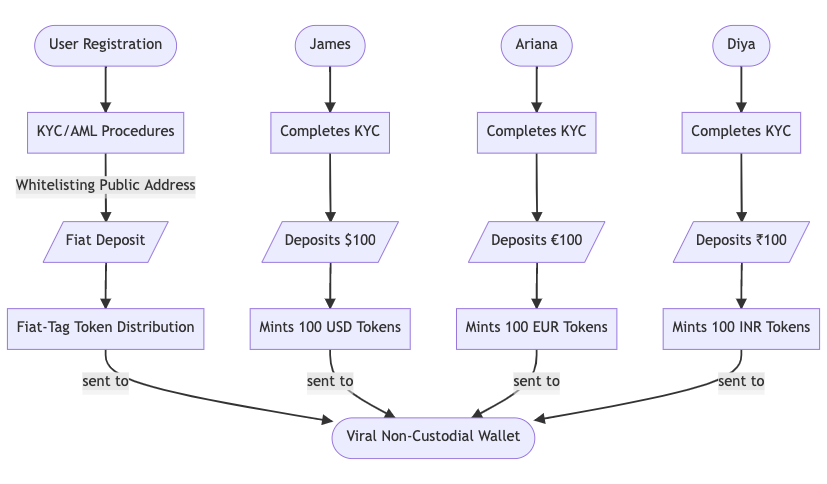
\includegraphics[width=10cm]{user-deposit}\\
\caption{User Deposit and Fiat-Tag Token Distribution}
\end{center}
\end{figure}


\begin{comment}%mermaid
graph TB
    
    A([User Registration])
    C[KYC/AML Procedures]
    D[/Fiat Deposit/]
    E[Fiat-Tag Token Distribution]
    A-->C--Whitelisting Public Address-->D-->E

    F([James])
    G[Completes KYC]
    J[/Deposits \$100/]
    K[Mints 100 USD Tokens]
    F-->G-->J-->K

    L([Ariana])
    M[Completes KYC]
    N[/"Deposits €100"/]
    O[Mints 100 EUR Tokens]
    L-->M-->N-->O

    Q([Diya])
    R[Completes KYC]
    S[/"Deposits ₹100"/]
    T[Mints 100 INR Tokens]
    Q-->R-->S-->T


    P([Viral Non-Custodial Wallet])
    E & K & O & T--sent to-->P
\end{comment}


Atomic Exchange from token to token\\

Makers as Sellers\\

\begin{figure}[H]
\begin{center}
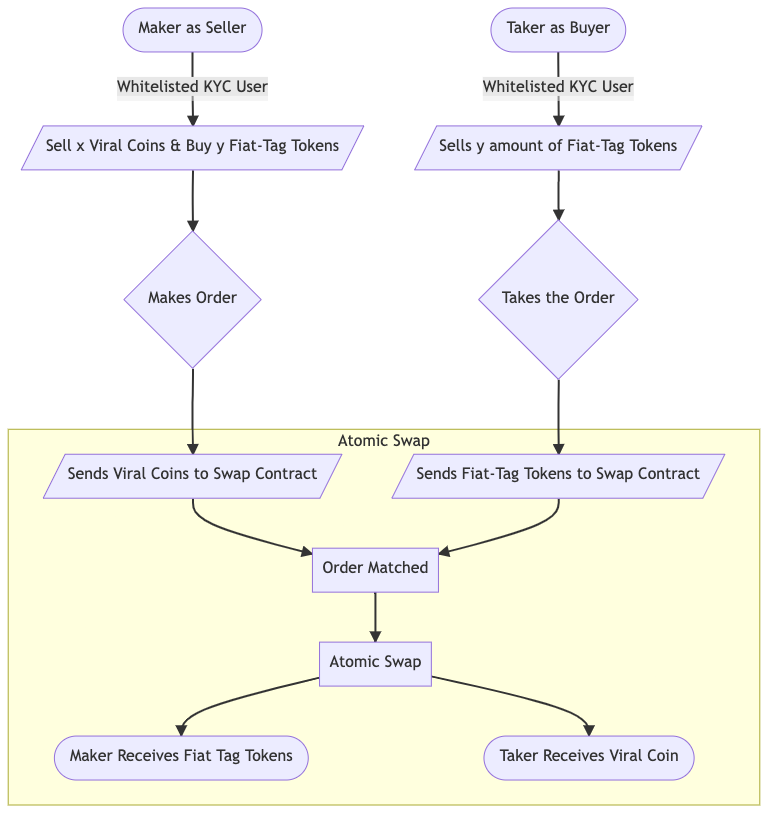
\includegraphics[width=9cm]{maker-as-seller}\\
\caption{Maker as Viral Coin Seller}
\end{center}
\end{figure}

\begin{comment}%mermaid graph
graph TB
    
    0([Maker as Seller])
    0--Whitelisted KYC User-->H
    H[/Sell x Viral Coins & Buy y Fiat-Tag Tokens/]
    H-->D{Makes Order}
    subgraph Atomic Swap
    E[Sends Viral Coins to Swap Contract]
    W[Sends Fiat-Tag Tokens to Swap Contract]
    S[Order Matched]
    U[Atomic Swap]
    F([Maker Receives Fiat Tag Tokens])
    V([Taker Receives Viral Coin])
    end
    D-->E
    X-->W
    E & W -->S
    S-->U
    U-->F & V
   
    X{Takes the Order}
    Y[/Sells y amount of Fiat-Tag Tokens/]
    Z([Taker as Buyer])
    Z--Whitelisted KYC User-->Y-->X

\end{comment}

Makers as Buyers\\


\begin{figure}[H]
\begin{center}
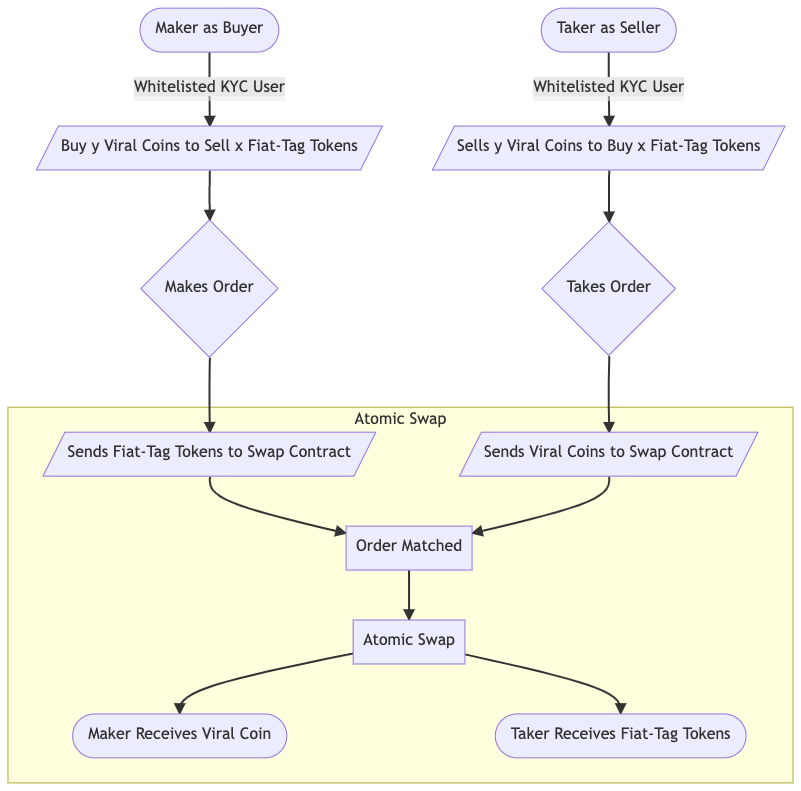
\includegraphics[width=9cm]{maker-as-buyer}\\
\caption{Maker as Viral Coin Buyer}
\end{center}
\end{figure}


\begin{comment}%mermaid graph
graph TB    
    0([Maker as Buyer])
    0--Whitelisted KYC User-->H
    H[/Buy y Viral Coins to Sell x Fiat-Tag Tokens/]
    D{Makes Order}
    H-->D
    subgraph Atomic Swap
    E[/Sends Fiat-Tag Tokens to Swap Contract/]
    W[/Sends Viral Coins to Swap Contract/]
    U[Atomic Swap]
    S[Order Matched]
    F([Maker Receives Viral Coin])
    V([Taker Receives Fiat-Tag Tokens])
    end
    D-->E
    X-->W
    E & W -->S
    S-->U
    U-->F & V
   
    X{Takes Order}
    Y[/Sells y Viral Coins to Buy x Fiat-Tag Tokens/]
    Z([Taker as Seller])
    Z--Whitelisted KYC User-->Y-->X
\end{comment}

Withdrawal of Fiat\\

\begin{figure}[H]
\begin{center}
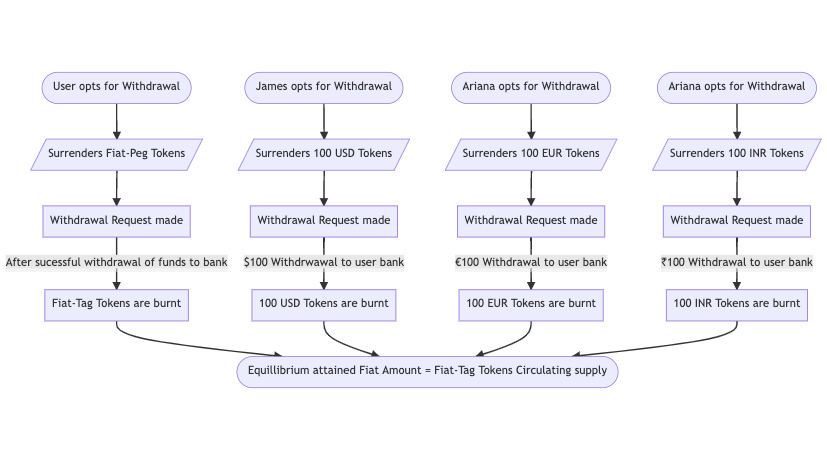
\includegraphics[width=10cm]{withdrawal}\\
\caption{Withdrawal of User Fiat Funds}
\end{center}
\end{figure}


\begin{comment}%mermaid graph
graph TB
    
    A([User opts for Withdrawal])
    B[/Surrenders Fiat-Peg Tokens/]
    C[Withdrawal Request made]
    D[Fiat-Tag Tokens are burnt]

    A-->B-->C--After sucessful withdrawal of funds to bank-->D

    E([James opts for Withdrawal])
    F[/Surrenders 100 USD Tokens/]
    G[Withdrawal Request made]
    H[100 USD Tokens are burnt]

    E-->F-->G--\$100 Withdrwawal to user bank-->H

    I([Ariana opts for Withdrawal])
    J[/Surrenders 100 EUR Tokens/]
    K[Withdrawal Request made]
    L[100 EUR Tokens are burnt]

    I-->J-->K--"€100 Withdrawal to user bank"-->L

    M([Ariana opts for Withdrawal])
    N[/Surrenders 100 INR Tokens/]
    O[Withdrawal Request made]
    P[100 INR Tokens are burnt]

    M-->N-->O--"₹100 Withdrawal to user bank"-->P

    D & H & L & P -->Q

    Q([Equillibrium attained Fiat Amount = Fiat-Tag Tokens Circulating supply])
\end{comment}

\textbf{Fee Structure}\\

Viral Semi-CEX takes very less percentage of fees comparing to other popular centralized exchanges. Viral takes fees based on deposit, withdrawal and trade. These fees doesn't include the network fees paid to the Viral Smart Chain which will be included seperately. Since Viral Smart Chain doesn't take gas fees and takes a very minute amount of base fee \$0.0005 and a transfer fee of 0.05\% it will not affect the users trades. The exchnage fees are listed below\\

\textbf{Deposit fees}
\begin{enumerate}[leftmargin=+0.2in]
\item \textbf{Deposit Fee}: Fized 0.1\% excluding credit/debit card or bank transfer fee
\item \textbf{Mint Fee}: Fee charged for minting new fiat-tag tokens .i.e., typically \$0.0005
\end{enumerate}

\textbf{Trade Fee}
\begin{enumerate}[leftmargin=+0.2in]
\item \textbf{For Market Makers} the trade fee will be \textbf{zero}. Only the network fees (base fee + transfer fee) will be leaved.
\item \textbf{For Marker Takers} the trade fee is fixed to \textbf{0.2\% }excluding the network fees to begin the trade.
\end{enumerate}

\textbf{Withdrawal Fee}
\begin{itemize}[leftmargin=+0.2in]
\item \textbf{Withdrawal Fee}: Fixed 0.1\% excluding credit/debit card or bank transfer fee
\item \textbf{Burn Fee}: Fee charged for burning fiat-tag tokens .i.e., typically \$0.0005
\end{itemize}



\textbf{Makers Incentives}
\begin{enumerate}[leftmargin=+0.2in]
\item \textbf{Zero-Fee Trades}: Viral Semi-CEX offers zero fee trades for market makers
\item \textbf{Rewards from Takers Commission}: 10\% of the takers commision (0.2\%) will be rewarded to market makers as an incentive for providing liquidity. 
\end{enumerate}


\textbf{Fiat-Markets}\\

At the beta launch of the Viral application we will be launching with Top 7 Fiat Currency with the highest market cap listed to buy/sell Viral Coins. Since for every circulating Fiat-Tag Tokens, the funds will be holded through a fiat-reserve bank. This requires local effort to go through regulation processes of the region. So Viral will be adding new fiat-currency listings according to the amount of requests we receive. The list of 7 fiat currencies are
\begin{enumerate}[leftmargin=+0.2in]
\item USD - United States Dollar
\item EUR - Euro
\item JPY - Japanese Yen
\item GBP - Pound Sterling
\item KRW - South Korean Won
\item INR - Indian Rupee
\item CAD - Canadian Dollar
\end{enumerate}
Currently Viral operates as a stand alone application for the users to make use of cryptocurrencies through our decentralixed social media, we provide users solution to buy \& sell only Viral Coins at the current scenario. There is plans to add more wrapped-crypto pairs in the upcoming future such as vBTC, vETH, vSOL, vMATIC to hold cryptocurrencies in a single non-custodial wallet and trade in with fiat currencies at ease.


Conclusion\\

\subsection{Viral Decentralized Exchanges}

Decentralized exchanges (DEX) are a type of cryptocurrency exchange that allows for direct peer-to-peer cryptocurrency transactions to take place online securely and without the need for an intermediary or a custodian, unlike Centralized exchanges. Decentralized exchanges are simply a set of automated smart contracts (code). They establish the prices of various cryptocurrencies against each algorithmically and use “liquidity pools” — in which investors lock funds in exchange for interest-like rewards — to facilitate trades. While transactions on a centralized exchange are recorded on that exchange’s internal database, DEX transactions are settled directly on the blockchain itself. There will be no custodian or any services which need to be maintained by a certain company to run a truly decentralized crypto exchange.DEXs are usually built on open-source code, meaning that anyone interested can see exactly how they work. That also means that developers can adapt existing code to create new competing projects — which is how Uniswap’s code has been adopted by an entire host of DEXs with “swap” in their names like Sushiswap and Pancakeswap.\\

\textbf{Automated Market Makers}

An automated market maker (AMM) is a type of decentralized exchange (DEX) protocol that relies on a mathematical formula to price assets. Instead of using an order book like a traditional exchange, assets are priced according to a pricing algorithm.This formula can vary with each protocol. Most AMMs usesa constant product formula: $x * y = k$, where $x$ is the amount of one token in the liquidity pool, and $y$ is the amount of the other. In this formula, k is a fixed constant, meaning the pool’s total liquidity always has to remain the same. Liquidity providers (LPs) add funds to liquidity pools. In return for providing liquidity to the protocol, LPs earn fees from the trades that happen in their pool. LPs deposit an equivalent value of two tokens – for example, 50\% of Token A and 50\% of Token B to the A/B Lquidity pool.\\

\textbf{Pros of AMMs}
\begin{enumerate}[leftmargin=+0.2in]
\item \textbf{No KYC Procedures}: Decentralized exchanges are similar to peer-to-peer exchanges but rather taking from an individual the user can withdraw funds from a trustless liquidity pool that requires no ID verification and other complex processes
\item \textbf{Secure} : DEXs are secure as the funds are withdrawn, deposited and held on-chain through smart contracts that is secure and immutable
\item \textbf{Non Custodial}: Liquidity Providers can provide liquidity and withdraw them whenever they need to, making it a non-custody protocol where user's funds will be held on a smart contract rather than a central custodian.
\item \textbf{Zero Manipulation}: Since user's funds are stored in a trustless manner, the smart contracts cannot freeze any account, transfer data to anyone nor manipulates price like a centralized exchange
\end{enumerate}

\textbf{Cons of AMMs}
\begin{enumerate}[leftmargin=+0.2in]
\item \textbf{Scalability}: Various DEXs are suffered from network congestions which delays the execution of trades. This is been solved by making DEXs on top of scalable high throuoghput blockchains, but the DEXs are limited to the scalability of the blockchain itself and cannot scale on it's own.
\item \textbf{Price Impacts}: Price impact is the influence of user's individual trade over the market price of an underlying asset pair. It is directly correlated with the amount of liquidity in the pool/Automated Market Maker (AMM).
\item \textbf{Limited Functions}: AMM based DEXs offers only to execute buy and sell orders and doesn't offers advanced trading features like limit orders aren't available on current exchanges.
\item \textbf{Volatility}: As price impacts being created, on an illiquid trading pair the volatility always reach new highs to stabilize the constant $k$ in the constant product formula $x*y=k$ to satisfy demands. This creates high volatile market while user's only use DEXs go for high liquid, low volatile market.
\item \textbf{Impermanent Loss}: Impermanent loss describes the temporary loss of funds occasionally experienced by liquidity providers because of volatility in a trading pair. Liquidity Providers suffer negative returns comparing to holding tokens outside the pool. Volatility and Price Impacts are the major aspects of impermanent loss. The loss becomes permanent if a provider decides to withdraw their liquidity from the pool.
\end{enumerate}

\textbf{Problem 1 : Price Impacts \& Volatility in AMMs}\\

The difference between the current market price and the price a user will pay to perform a swap in a decentralized exchange is known as Price Impacts. This happens when the ratio of the assets in the pool changes where one asset is more liquid and another is illiquid. When a large swap is conducted a maximum portion of the swapped asset is erased from the liquidity pool, supplying more of the provided asset, to maintain the $k$ of the constant product formula $x*y=k$ the smart contract will ask for a increased supply of tokens to balance the $k$. This will create a impact on the current price, making the trade much more expensive than centralized trades and spiking the volatility of the pool.\\



For example\\

Two Coins $X$ and $Y$\\


\textbf{Pool Info/Before Swap}:
\begin{itemize}[leftmargin=+0.2in]
\item Before Swap $X$=20
\item Before Swap $Y$=45,000
\item Constant Product $K=X*Y$ = 900,000 
\item Before Swap Price $M=\frac{Y}{X}$ = 2,250 
\end{itemize}

\textbf{Trade $n$}: $n$= 9,000 y for x\\

\textbf{After Swap}:
\begin{itemize}[leftmargin=+0.2in]
\item After Swap $Y_n$=54,000 
\item Constant Product ($K$) = 900,000 (Stays Same)
\item After Swap $X_n=\frac{K}{Y_n}$ = 16.666  
\end{itemize}
\textbf{Results}:
\begin{itemize}[leftmargin=+0.2in]
\item Received $X_f={{X}-{X_n}}$ = 3.334 
\item Price paid per X / After Swap Price $M_n={\frac{n}{X_f}}$  = 2,699  
\item \textbf{Price Impact} $P={\frac{M - M_n}{M}*100}$ = \textbf{19.95\% }
\end{itemize}


\textbf{Conclusion}:\\

To take 9,000 Y Tokens from XY Pool having 20:45000 Tokens, user have to pay \textbf{19.95\% more} than the market price. \textbf{Market Price = 2,250} , \textbf{User Price = 2,699}\\


Huge price impacts happens only in pools that has less liquidity when a maximum percentage of a token in a pool is withdrawn. These price impacts are being neutralized by arbitrage traders who buys token at lower prices on other exchanges and sell the same token high on decentralized exchanges which will has a maximum price impact, these arbitrage traders will continue to make trades for profits until the market price is achieved. Although arbitrage traders are available to minimize the price impacts, users cannot always wait for the arbitragers to stabilize the pools. DEX aggregators offer users a better solution by buying the token across all pools in order to minimize price impact on each one of them. Instead of spreading the trade over time in a single market, this order executes at once, spread over many possible markets. Aggregators also command substantially higher gas costs than a single trade, similar to splitting trades manually. To conclude there are different secondary solutions that minimizes the price impact through secondary trades (trades after the price impact maximizes), the first trader after it neutralizes will always execute orders with price impacts and slippage of prices while multiple trades happen in the middle.\\

\textbf{Problem 2 : Limited Functions}\\

Order book centralized exchanges offers advanced trading features such as limit orders where traders can bid and ask at different prices from the current market prices. DEXs doesn't offer limit orders and only offers instant market orders with a possible price impact. Order book exchanges are better in terms when it comes to live exchanges and better prices for buying and selling. AMMs has its own benefit compared to order books by providing liquidity at anytime regardless of number of orders.\\

\textbf{Problem 3 : Impermanent Loss}\\

Impermanent loss is the most common loss a liquidity provider experience and a risk of using Automated Market Maker (AMM) based Liquidity Pools. Impermanent loss deals with pairs of the liquidity pools, usually while contributing to a liquidity pool a liquidity provider shall equally provide both tokens according to it's market price that will determine the liquidity providers share of the pool in percentage. For example in a pool of XY Tokens for every X token \$100 tokens of Y should be provided taking Y token as a Stable Coin with Y=\$1, when a LP provide 1:100 worth \$200 to the pool with a final ratio of 10:1000 has 10\% of the pool where the LP will be rewarded extra with the transaction fees (usually 0.3\%) according to the percentage the the LP holds. To represent his liquidity the LP will be offered with LP Tokens of the specific pool which the LP can claim and withdraw his tokens.\\

When trades happens the volatility of the two pairs is a nightmare to LPs due to changes in prices that leads to impermanent losses. Impermanent losses are not permanent until the LP withdraw his pool's liquidity. From the above example after the LP provided XY Tokens with 1X = 100Y if the price of X token appreciates to 1X = 400Y, the ratio of the pool would haved changed to 5:2000 maintaining the constant of total liquidity. When the LP withdraws his tokens from the pool he is entitled to his 10\% of funds withdrawing 0.5X and 200Y which totals to \$400. The LP made a profit of \$200, but would have gained more by simply holding the funds of 1X and 100Y worth \$500. The losses compared to holding and providing to a liquidity pool is often termed as impermanent loss but sometimes will be substituted by trading fee rewards. Effects of huge price volatility and impacts creates impermanent losses of LP's funds.\\

\textbf{Problem 4 : Scalability of DEXs}\\

Decentralized exchanges suffer greater scalability issues during frequent network congestions of blockchains. The scalability of DEXs is directly related to the scalability of blockchains. Without a highly scalable blockchain DEXs cannot prepare for a mainstream adoption where trading volume would increase by radical margins.\\

\textbf{Solution to Current Risks}\\

Current AMMs gives the opportunity for non-simultaneous series of buys and sells where two traders can buy A tokens freely which will increase the price impact thereby making the pool's token price to change drastically compared to the original market price. To eliminate price impacts for the next buyer (buy-buy trade) the following swaps (next swap order) should be opposite to the previous swap (sell) i.e., While first swap takes A tokens for B , the following trade should be taking B tokens for A, thereby minimizing price impact by stabilizing the pool for the next (buy) traders. A simultaneous matching of buyers and sellers can minimize the price impact for the next set of buyers and sellers. This matching is in centralized exchanges are done through order books where it matches traders for their input price .i.e, a limit order. The solution is to maintain a swap book on top of the liquidity pool to match buyers and sellers to maintain the stability of the pool and eliminate price impacts.\\

\begin{figure}[H]
\begin{center}
\caption{Flowchart of Explaining current AMM orders vs Required Orders}
\end{center}
\end{figure}

While conducting an alternate(buy-sell) swap, it leaves significant price impacts on either of the trades for maintaining the $k$ in the Constant Product Formula $x*y=k$, it will not be useful to minimize the price impacts by doing two trades one after each other. Also when two trades match it is best in case to make a decentralized atomic swap instead of taking from a Liquidity pool that will revert to it's previous pool price before the trade. This comes to a conclusion that Traders with matching swaps doesn't provide any results for reducing price impacts, changing the pool's price to market price, etc. \\

\begin{figure}[H]
\begin{center}
\caption{How matching buyer and seller won't change pool price and create impacts}
\end{center}
\end{figure}

To give solution to all the existing AMM risks and problems we should be allowing traders to only withdraw if they match with their corresponding opposite trader (buy-sell) while changing the traders buy/sell amount to change the pool's price to market price by traders acting as a smaller liquidity providers. \\

\textbf{Intro to Viral DEX}\\

Viral DEX is a Liquidity Pool exchange that matches buyers and sellers through it's swap book on top of it's Liquidity Pools while automatically rebasing the pool to it's live market's price thereby minimizing price impacts and proving faster and scalable trades using its micro-pool architecture\\

\textbf{Micro Pool Architecture}\\




Micro Pool Architecture\\
Liquidity Providers\\
Advanced Trading\\
Benefits of Viral DEX






\subsection{Wallet Transfers \& Viral Name System}

\subsection{Custodian Services}

\subsection{Other Wallet Features}

\textbf{QR Pay}\\

The need for faster transactions is rising higher every year and new technologies have been introduced such as NFC, Scan Code, etc. Since Viral Wallet is a crypto wallet, it will be hard for people to use a public address to send and request Viral Coins or other cryptocurrencies to Merchants using the Smart Wallet . QR Pay is a feature to be added on the Smart Wallet to facilitate faster recognition of seller’s wallet address and the amount to be transferred by scanning a simple generated QR Code through Viral Application. This QR Pay will come when the user doesn’t know their username and want to request money from a nearby person. This will be helpful for businesses to collect payment from users swiftly by entering the amount needed to be paid.\\

\section{Child Platforms}

\subsection{Content Moderation Platform}

Centralized social media holds the administrator rights of users’ data which circulates in their platform and also misuses their authority by deleting or expelling a certain user from posting content. This effectively increases the chance of eliminating individual rights, dealing with governments, and most importantly losing the trust of the people. Usually, content moderators on existing social platforms will be held responsible for removing illicit content whereas sometimes due to a centralized approach these moderators are told to filter independent content posted by creators on certain topics where the companies works with the governments sideways. This is why a decentralized community such as ROV is needed for the Viral Network to automate the process by giving administrative rights of the source-uri of contents inside the Viral-Alpha Application to a swarm of moderators which is going to be the key for independent content and removal of explicit contents in a faster and democratic way possible.\\

ROV is an abbreviation for Republic of Viral, a decentralized community-based organization inside Viral Network to govern, filter out reported contents, give support to users, verify VIPs, vote on involvements of community members, etc. The Community is solely developed to bring a decentralized way of allowing a network of administrators under a voting mechanism to remove NSFW, spam content in the Viral Network, and aims to create a cleaner social media while restraining the power of censorship resistance. ROV is designed for curators to work as employees of an organization with a common goal with maximum trust and anonymity. This decentralized way effectively reduces the opinion of a single person, an entity’s founder, and any external influence where the community only decides which is better for the platform. ROV eliminates the need for a centralized entity to run a social platform that holds the power of democracy while ignoring censorship resistance. \\

Moderation and Manual Removals

Type about we focus on the source rather than the full post\\
Type about how Viral has both IPFS Public and IPFS Private\\
Removal of Content from Viral IPFS-Clusters\\

\begin{comment}

In Decentralized systems, it is hard to censor or remove content circulating in the platform. The files won’t be stored in a single server but Viral have paved a way where the content removal happens at its best without an organization or an administrator but as a series of votes and process of all stabilizers (IPFS Clusters) to remove the certain file from all the peers which hosting the file for the viral network. After the Content is decided to remove (after the Poll Ends), immediately the stabilizers (miners) who hosts the content on their desktop, laptops, servers will be notified to remove the content from the IPFS clusters. This is achieved by making a private IPFS cluster separately for Viral Network to hold files. Since the mobile peers which hold the content will be clearing every 30 mins, the reported content will not be hosted anywhere on the platform removing it completely from the network of decentralized servers.\\

\end{comment}

Timer for Removals\\
To ensure faster removals and counter the delay of manual approach of votes calculation, after content is reported it will be directly posted on ROV’s Application where the voting poll for the specific post timer will run according to the category’s emergency for removal. This ensures faster content removals in no time, where it takes 24 – 48 hours for a centralized social media entity. We have listed out the major categories and timings for reporting illicit content in Viral. \\

\begin{itemize}[leftmargin=+0.2in]
\item Spam or Fraud – 2 hours
\item Bullying or Hate Speech – 45 mins
\item False Information – 1 hour
\item Sexual Harassment - 30 mins
\item Nudity – 30 mins
\item Violent or Disturbing – 30 mins
\item Something Else – 2 hours
\end{itemize}

Algorithmic Automated Removal Methods\\

Additionally, to improve faster removals we will be rolling out another AI feature that finishes the poll timer if the votes are more than 10 and 95\% have voted to remove content or keep content. This effectively eliminates the possibility of waiting to remove the content till the timer ends, if the post is in a high state of emergency to remove. There will be an AI feature also to filter out pornographic content on the platform automatically without any votes.\\

Formula for Ending Timer\\

Separate Application

ROV will be having a separate Mobile Application for curators and moderators to easily vote for reported contents using swipe methods similar to dating apps such as Tinder. Since ROV is a restricted content application it will not be available on the Play Store and App Store. The Mobile Application will be only available on Android as a 3rd Party App and won’t be available for iOS devices due to their security policies.\\

Process of Polls\\


\begin{figure}[H]
\begin{center}
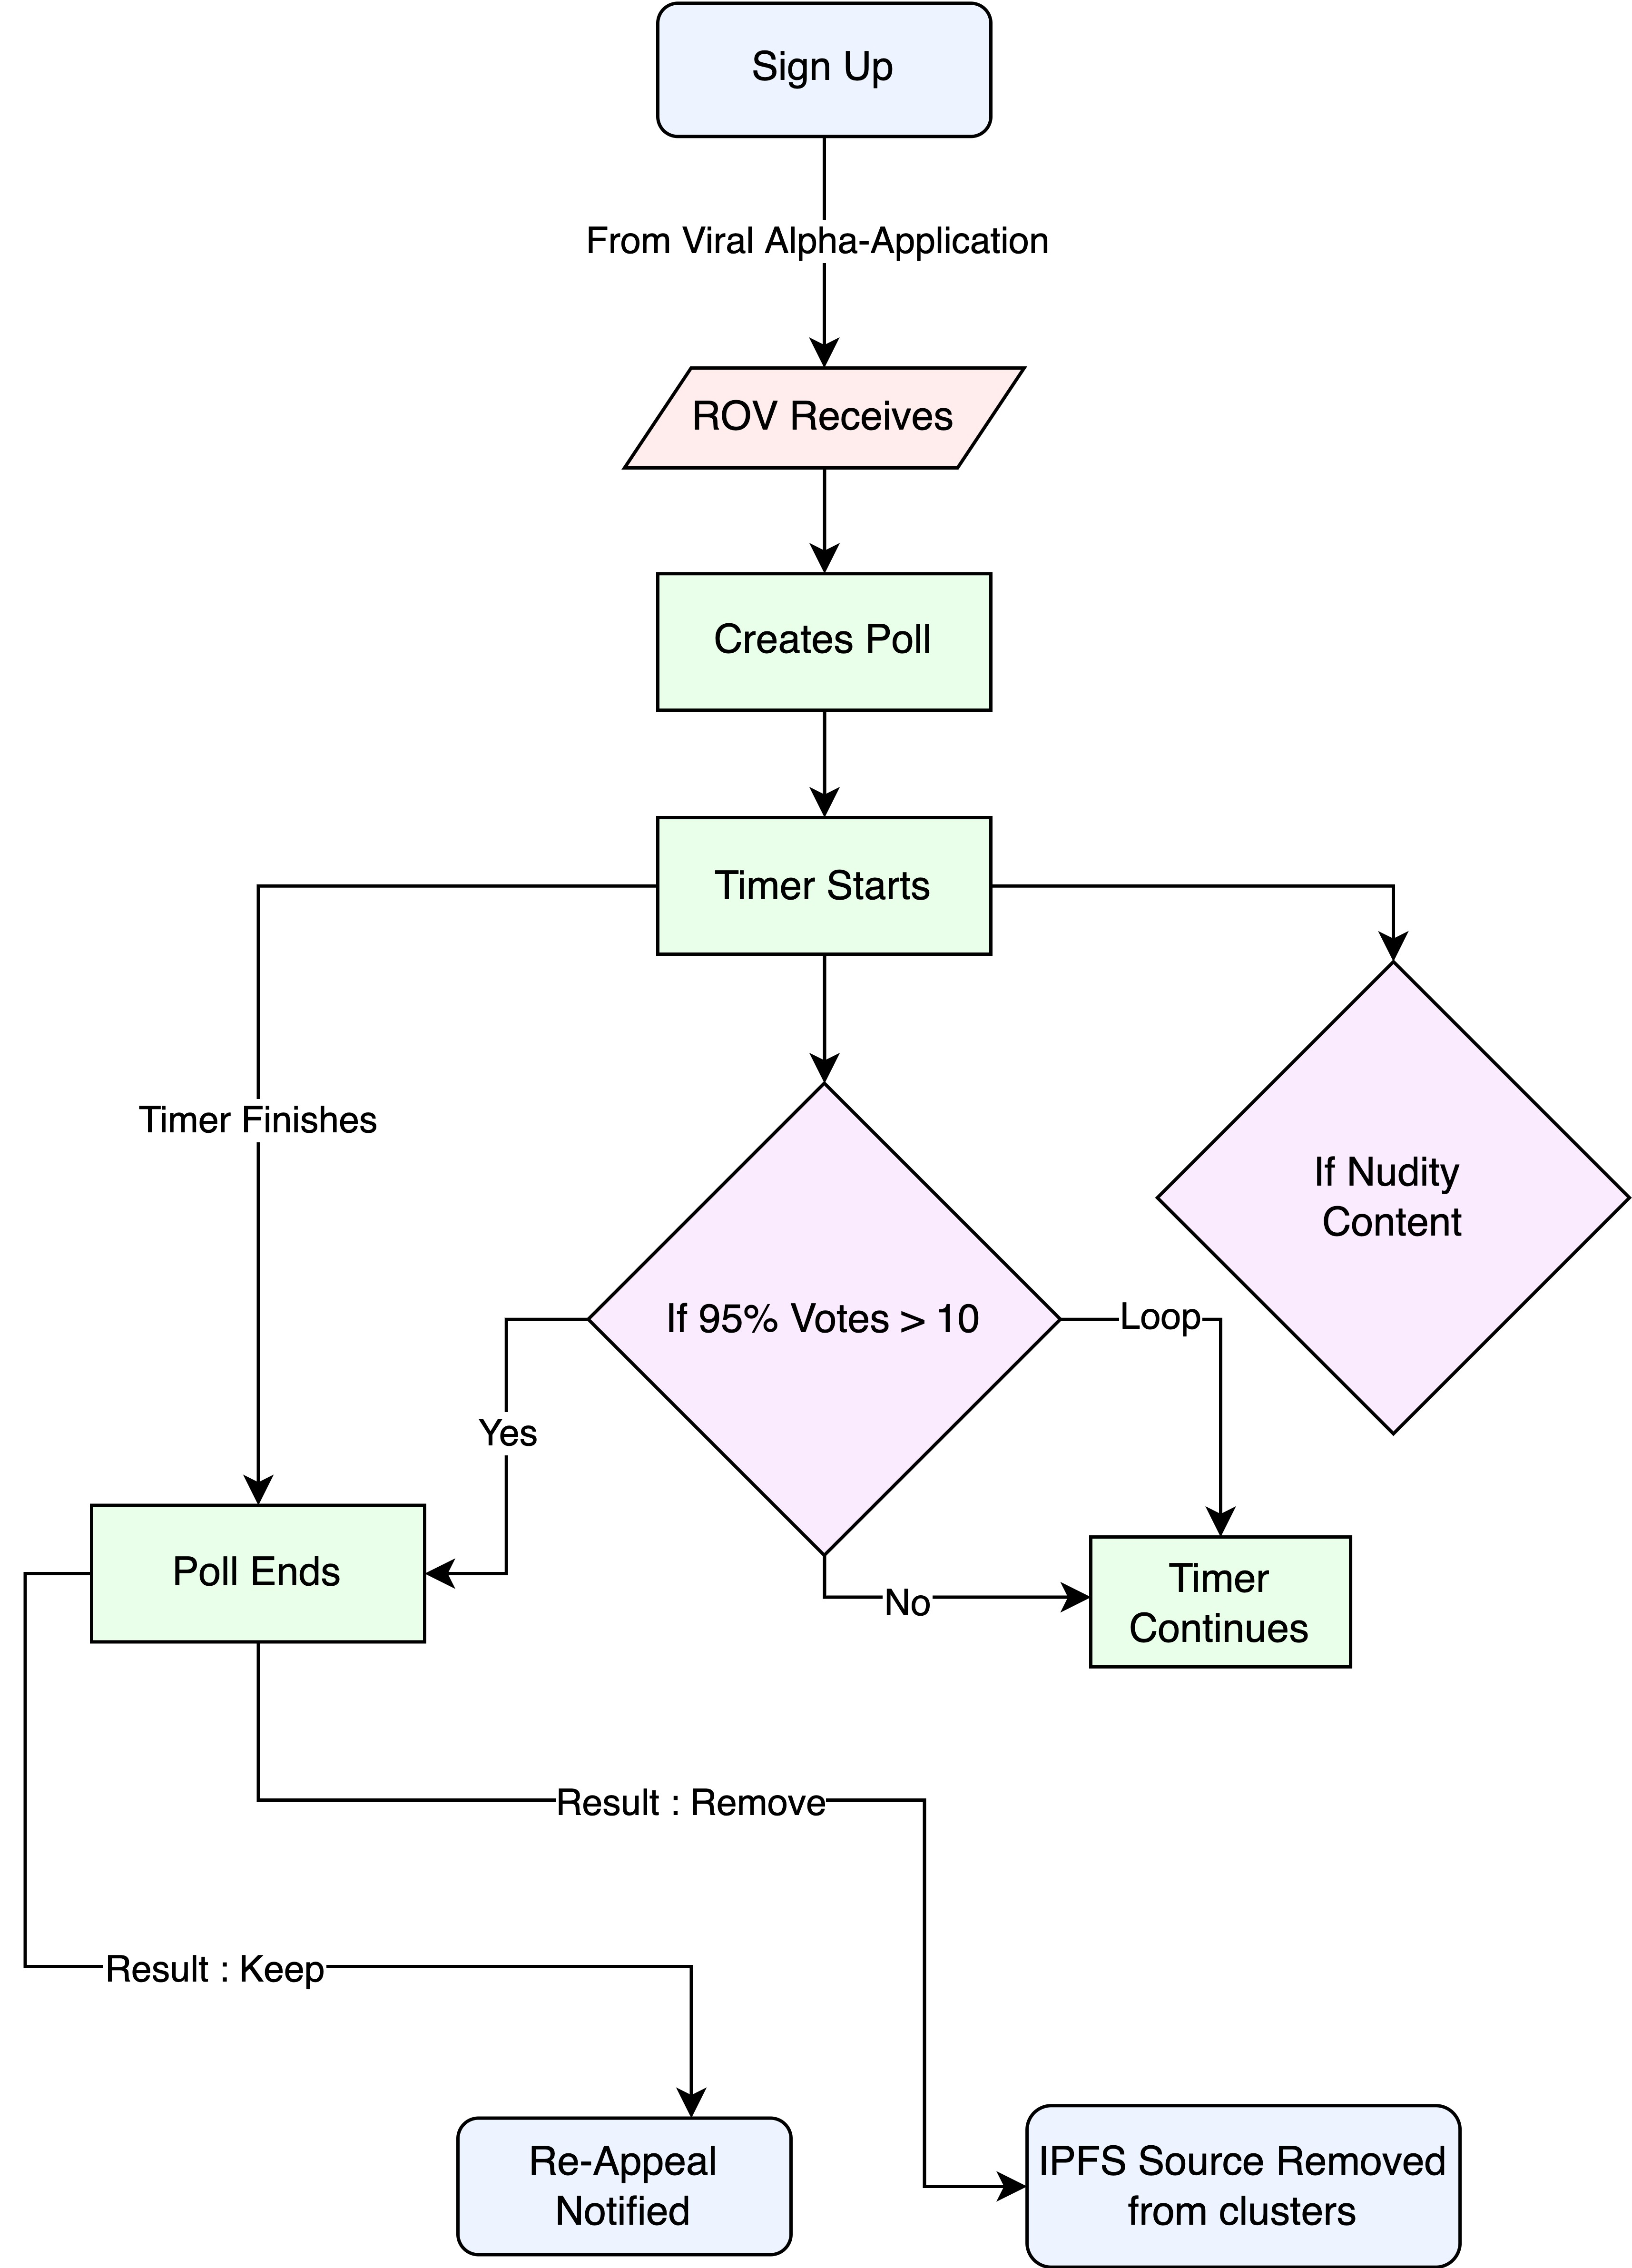
\includegraphics[width=8cm]{rov-poll}
\caption{Glimpse of ROV Process}
\end{center}
\end{figure}


\begin{comment}%rovgrpah

%mermaid graph https://mermaid-js.github.io/

flowchart TB

A([User Reports])--From Viral App-->B[/ROV Receives/]
B-->C
C[Creates Poll]-->D[Timer Starts]
D-->E{If 95% Votes >10}
D-->|Timer Finishes|H
E--no-->G[Timer Continues]
E--yes-->H[Poll Ends]
G--loop-->E
H-->|Result: Keep|I([Re-Appeal Notified])
H-->|Result: Remove|J([IPFS source removed])

\end{comment}


Continuous Removal Caution to change to private account\\

Re-Appeals\\

A unique feature of ROV given to the users of Viral to re-appeal or re-report against the decision of voters while giving an explanation where the ROV curators can again vote to keep the content again or remove based on the explanation given by the user who re-reported. The timer for re-appeal is 5 hours per post where if votes are more than 25 and 90\% opt again to keep or remove the timer will end prematurely.\\

Limitations\\

Private Accounts\\

Viral’s content reports are only applicable to public accounts. Viral’s vision to bring complete privacy and security to private accounts which are exempted from being reported. ROV curators will not moderate, nor involve to view the contents of secured private accounts. Thus, it leaves decisions in the hands of followers whether to view their content or not. \\

IPFS Public Node \\

Criteria to Join\\

Viral DAO token holders will be given privilege to run ROV as curators and so on\\

Eliminating Bad Curators\\

To eliminate biased curators we will be bringing a safe mechanism to filter out bad curators in the community using a feature called positive/negative points. Every single poll will contain two options for the curators to select, “Remove” or “Keep”, the poll results are based on the majority’s decision. When a vote for a poll and falls under the majority’s vote the curator will receive a Positive point, if the curator is on the minority side, which is the losing side he/she be getting a Negative point. Each of the positive and negative points will be added to his profile. An algorithm will run to take the percentage of both points, where if the negative point falls above 30\% to the positive point, his ROV account will be suspended for a couple of days. We have deciphered the factors where there could be no bad actors in the community. There will be records to everyday's positive and negative points. \\

This Positive/Negative points suspension factor will be running after every single vote after the poll finishes. Some factors determining the suspension are\\

If Negative Point is 30\%- 40\% to the Positive Point – Account suspension for 3 days\\
If Negative Point is 40\%- 50\% - Account suspension for 6 days\\
If Negative Point is more than 50\% - Account suspension for 12 days\\

We have also made factors to suspend an ROV account forever based on the number of suspensions they get on their account. The factors are\\

 20 times 3 day suspension \\
 10 times 6 day suspension\\
 3 times 12 day suspension\\

There will be a test-net and live-net to practice voting at its best\\

Example : \\

User A: Day 26; Positive – 234; Negative – 55; Result: More than 20\%: Suspension for 3 days\\
User B – Day 30; Positive – 523; Negative – 343; Result : More than 50\% : Suspension for 12 days\\


Community Help \& Support\\

ROV will be having a separate section for community help \& support, where ROV curators can easily offer their support to Viral users by providing them answers for their queries through the application. The Curators will act as support persons for their issues and thereby providing answers for their problems. It will be a decentralized substitute for centralized customer support. Since the curators cannot offer custom support by an admin staff in a centralized company rather, they can offer support for their questions regarding the usage of the application. For every contribution by the curators, they’ll receive their fair share of rewards.\\


Verification of Accounts of Celebrities\\

ROV curators also will be responsible for several actions on the decentralized platform, one of it's the "Verification of Accounts". Since Viral doesn’t take a single byte of data, we won’t be requesting any country’s identification information like other centralized social medias, it is up to the curators to opt for giving a verified tick for the VIPs on the viral platform.\\

Data to Disclose\\
About Verified NFT\\
Flowchart\\
Regional Voting\\


Requesting ROV\\

Since ROV is regarded as a DAO (Decentralized Autonomous Organization) we make sure others request ROV for a specific task, poll, support, etc. This feature will be given only to verified profiles where they can write to ROV in any matter where the curators can come collectively to help regarding the issue. This will help VIPs, Governments to write to ROV curators which will be displayed on their feed where they can take necessary actions for it. \\

Rewards for Contribution\\

ROV users’ wallets will be connected to their username where every day according to their contribution the Viral Coins will be allocated every 24 hours and will be airdropped to their wallets where they can collect manually. According to the features and intensity of work will be appointing a pointing structure in the development phase of the ROV application\\

Rewards according to daily positive points\\

\subsection{Developer Platform}

Story\\

Viral Dev-Space is a platform for developers to develop, communicate together with other experts, and receive rewards for their contribution to the Viral Open-Source applications and future development plans of the public and the Viral DAO. The Space for developers is created to decentralize and automize the Software Research \& Development sector of Viral Applications in an efficient way by providing rewards in Viral Coins through unbiased voting based on the intensity of their contribution and popularity in the development community.\\

Viral will be providing an opportunity for all developers regardless of their educational background, region, and language to work on improving the viral decentralized applications on fields such as security, interoperability with other social giants and also to make the application bug-free while providing new updates to the beta software which will be available as an Open-source repository. Giving new opportunities to develop for an upcoming massive social network will pave a way for fastening the development process by using the potential of mass development techniques.\\


Short Benefits:
\begin{enumerate}[leftmargin=+0.2in]
\item Full Automation on Research \& Development
\item Potential of a bigger development community
\item New, Exciting Unknown Developments for the application
\item Shorter Time for fixing bugs and issues
\item The cost of Development is considerably low
\item Decentralized HR \& Rewards according to the contribution
\item Expedite the Development of Viral Future Plans
\item And many more advantages to receive a contribution for the application’s source code in trade for daily rewards
\end{enumerate}

Allocation of Rewards\\

The rewards are based on democratic voting where every developer will have their own project feed to appreciate the work of other developers. There will be an engagement feature to “Like” the contribution they’ve pushed to the code repository. After a developer makes a commitment to the repository by pushing his/her code to the master repository, their work will be posted on the project’s main feed. At the end of the day every 24 hours, the amount of likes every post received by the user profiles on all the projects will be taken to segregate the amount of rewards per developer. Refer Rewards section for detailed information on the segregation of total revenue separated for developers.\\

Application\\

Viral will provide a web application where developers can join, interact in development groups and receive rewards daily every 24 hours according to their contribution. This application will be maintained by Viral DAO. The App will serve as a community platform where any developer can choose their favorite preferences, communities, and development projects. Developers can choose the project of their preference by searching and also by opting for an interactive questionnaire to find out which project is suitable for them. After giving their preference they can choose the project they want to work in. The developer will have a limit of working on two projects at a time, where they can remove themselves from the project team and opt for other projects as well. This will ensure that developers will have an increased productivity and a higher success rate in specific projects.\\

App Features\\

\begin{itemize}[leftmargin=+0.2in]
\item Choosing preferred project
\item Collaborative Workspace for Developer Teams
\item Easy Work-Management
\item GitHub Account Integration
\item Private and Project Group Chats
\item Add New Projects to Dev-Space by providing a whitepaper
\end{itemize}

\subsection{Social Nodes}


\section{Global Reward Pool}

Story\\

Viral Rewards are daily rewards airdropped to every user on the decentralized platform who contributes towards running the platform. It includes Users, Stabilizers, ROV Users, and Developers. Since it is a decentralized platform, it requires no maintenance and authority by a centralized entity. The contribution of every single individual user is needed to run the platform seamlessly. We would be giving out rewards in form of Viral Coins for all the users who contribute to running the platform.\\

This includes\\
\begin{enumerate}[leftmargin=+0.2in]
\item App Users
\item ROV Curators
\item Social Nodes
\item Developers
\end{enumerate}


The Airdrops will be happening through automated smart contracts and off-chain transfers every day at 2 AM UTC. State Channels will be efficient for a huge transfer of Coins for millions of accounts receiving airdrops at once. The airdrops will be sent in a secured and anonymous way to ensure maximum privacy for every single user who is getting paid for their contribution on the Viral Decentralized Social Platform. \\

Viral Incentives are designed in such a way that every single contributor inside the network will get paid for their contribution through a democratic voting system and mathematically predicted points. These points prediction program will run on its own in Viral Smart Chain every day at 2.00 AM UTC to ensure fair rewards to each user without any influence, third-party recommendation, or external factors. For App users it would be according to the percentage of impressions they recieve on their content, for ROV curators it will be total Plus Points they add for their votes, for Social Nodes it will be based on their total contribution per day, for Developers it will be based on voting by other developers, by which the contribution will be rewarded by its own community-driven platform.\\

The 100\% percent of total daily revenue is distributed as \\
\begin{figure}[H]
\begin{center}
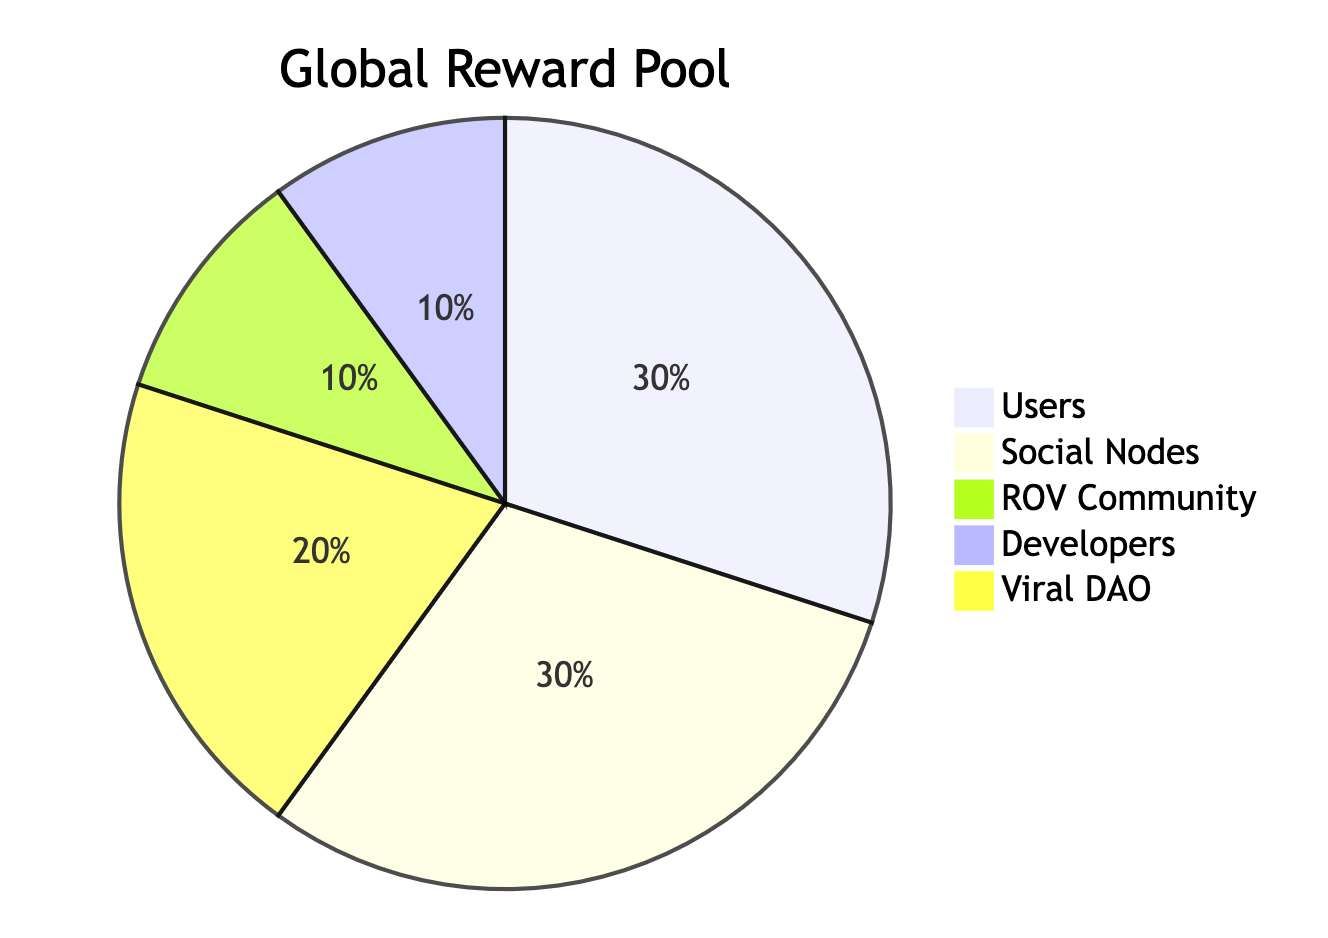
\includegraphics[width=9cm]{rewards}
\caption{Allocation of Daily Revenue in percentage}
\end{center}
\end{figure}

\begin{comment}%mermaid
pie

    title Reward Pool
    "Users" : 30
    "Social Nodes" : 30
    "ROV Community" : 10
    "Developers" :  10
    "Viral DAO" : 20
\end{comment}

30\% of rewards from the global reward pool is allocated to Application Users based on the total views/impressions users get on their profile. Impressions counts are agnostic to the type of content that is published in the Viral Application. Impressions/Views are a basic engagement of a typical social networking platform.This ensures every content creator on the platform will get rewards according to their reach, popularity, and usage they get for their content on the decentralized platform. This can keep content creators getting paid every day according to the traffic they receive on their profile/content they post.\\

Advantages\\

\begin{itemize}[leftmargin=+0.2in]
\item Creators can be able to create content expecting a reward for it
\item A fair share of rewards according to the popularity of the content.
\item Users will trust the platform which gives them 30\% of it’s daily collected revenue to every \item user without any centralized company meddling.
\item Encourages other platform users to join and receive rewards.
\end{itemize}


Segregation of Rewards\\

Global Impressions of all users will be taken to calculate each user’s individual percentage which will be required to allocate individual reward amount from the User Reward Pool.\\

Formula\\

Example\\

The distribution and analysis of coins for each User(Views-Based) will be done at 2.00 AM UTC every day. The users can collect their activity-based rewards manually within a stipulated period of 10 hours. Manual collection of rewards are specifically brought to ensure that the non-active users on the platform will not receive the rewards and only the people who contribute to the platform by being active will be receiving their rewards. The non-active users' coins will be sent to the burn address, where the coins will be burned.\\

If the user opts for transferring the rewards to a Non-Profit-Organizations it can be easily transferred directly to the user's preferred Charity. Viral will have a registration portal for Charities to Register their information and get verified to appear on the Application's Wallet. Other than the separated 20\% Viral DAO will not take or receive any additional coins, nor involve in any meddling process of taking away coins that are meant to give to the people who contribute and run the decentralized social media.\\

ROV (Contribution-based) - 10\%\\

10\% of rewards from the global reward pool is allocated to ROV (Republic of Viral), a content moderation community for the Viral Decentralized platform. There, curators will be filtering and voting posts to eliminate spam, inappropriate content which is reported by users and also govern the application's content in a democratic nature considering every curator's vote. This method of democratic voting community eliminates the power of a single individual to decide the type of content if it's violating the social media's posting guidelines. \\

This ensures rapid results in removing explicit content in a relatively short time without any hassles. In short, ROV is a decentralized autonomous organization to maintain Viral at its best. So, the curators should be rewarded by Viral Coins for their contribution to the network.\\

Advantages of ROV over Centralized Organization\\
\begin{itemize}[leftmargin=+0.2in]
\item Faster content removals
\item The decision of a single organization/person will be eliminated
\item A better-decentralized approach to centralized organizations
\item Will work in any time zone 24/7 without any hassles
\end{itemize}


How Segregation takes place\\

The segregation will be done at 2 AM UTC where the curator's Plus points for the day will be taken and the percentage of rewards will be determined using it. For every vote and every positive contribution they make the points will be increased in the ROV Profile where the curators will get their fair share of rewards considering the total points collected by all curators in 24 hours similar to the segregation algorithm of Users Views-based.\\

How will they receive\\

Every curator will receive their rewards directly to their wallets where they should collect them manually in a period of 10 hours.\\

Stabilizers (Serving based) - 30\%\\

Stabilizers are people running macro-servers in the viral decentralized network for storing and data transfer from one node to another node. It is similar to blockchain mining nodes but here the nodes will run IPFS Public Nodes, IPFS Cluster peer, Gun DB Relay server, WebRTC signaling server, and other several mini peers of other stacks simultaneously to provide faster data transfer, decentralization of data, higher encryption, better stability, etc. \\

Users can download the desktop software and run the program to become a social node for the Viral network and start earning rewards according to the data served for the network. In short, instead of buying centralized servers as other companies do, we will be providing a desktop software where any user can run the program in their desktop, laptop to become a server for the viral network to transfer, serve data on the decentralized platform and get paid by rewards every day to their wallet.\\

If the platform receives more social nodes\\
\begin{enumerate}[leftmargin=+0.2in]
\item More people will trust the social media
\item More relay peers equal faster transmission of data
\end{enumerate}


The segregation will take place at 2 AM UTC by taking the total number of data served from each technology stack's peer such as IPFS, GUN, WebRTC, and all other mini peers. The points will be given to stabilizers based on the percentage they served to total served by all stabilizers in the given 24 hours. \\

The stabilizers can able to receive their Daily rewards automatically to their wallets based on contribution, where the rewards have to be collected manually within the 10 hours stipulated window, in which the uncollected coins will be sent to burn address automatically.\\


Developers (Contribution-based) - 10\%\\

10\% of rewards from the global reward pool is allocated to Developers. Viral is an Open-source platform where developers contribute to development of the beta application which will be available as an open repository. To give rewards for developers' contribution to the decentralized platform and also to encourage developers by giving paid rewards to structure a better, safer, secure social media for the masses using collaborative work is the ultimate goal. By bringing mass development to life we can ensure that the people who run social media will be the product of millions of developers working every day for a common goal of a powerful social communication platform.\\

We will be linking developers' GitHub and viral accounts in a separate ROV-Dev Application in which the developers can contribute their work and get voted by other developers for rewards. The votes will determine their rewards where the max voted contribution will receive more viral coins than the min voted contribution on the beta-software.The developers are the backbone of Viral. Every single developer should be rewarded fairly for their work and the rewards should be determined by their fellow developers inside the community. Since there is no meddling of Viral DAO and its executives, the developer platform will be democratic, decentralized, and autonomous to keep the social media strong and secure in the most possible way. By rewarding developers, we can expect other developers to join the people-run social media.\\

Viral will give a better world to developers expecting a reward for their contribution and also engages a lot of developers into a small community to get most of the percentage from the allocated 10\% of daily revenue. This will encourage autonomous development of superior technology where all hands matter. \\

The segregation takes place every day at 2 AM UTC according to the votes they got for every single contribution to the beta platform and future plans. Every developer can vote on the done contribution by other developers on a special ROV-Dev Application. This will determine the popularity of the contribution and give fair rewards to each. The rewards will be sent to the Developers' wallets for manual collection which will be available to collect for a period of 10 hours every day.\\


\section{Viral DAO}

Story\\
Intro\\
Governance Models\\
Viral Smart Chain\\
On-Chain Governance\\
Staked Tokens\\
Viral Improvement Proposal\\
Addition of New Chains\\
Viral Ecosystem Governance\\
DAO Intro\\
List of Governing Platforms\\
Viral DAO Tokens\\
Holding Benefits\\
DAO Platform\\
DAO Revenue\\
Distribution and Dividends\\
Viral Operations Cost Structure Proposals\\
DAO Treasury and Decisions\\
Intial DAO Coin Offering\\
DAO Bylaws\\

\section{Viral Coin ICO}
Intro\\
Viral Coin Details\\
Token Distribution\\
Token Pre-Sale\\
Token Main-Sale\\
Token Alpha-Sale\\
Token Usages\\
Long Term Capital Gains\\
Incentives to Investors\\
Token Lockup Period\\
Investors Exit Strategies\\

\section{Development Roadmap}

Phase 1 - Beta Launch, Alpha Launch
Phase 2 - External Upgrades\\
Phase 3 - Internal Upgrades\\

\section{Phase 2}

\subsection{NFT L2 Solution}

\subsection{Viral DAO Platform and ICO}

\subsection{Viral Decentralized Ads}

\subsection{Influencer-Ad Platform}

Story\\

Viral Influencer Ad-Platform is a Gig-based marketplace where Content creators can post their ad-gigs under specific categories such as impressions, engagement, link clicks, etc to various businesses where they can purchase with the trust of the blockchain. After the promises of the gig are achieved the payment will be released to the influencers. This effectively reduces the unwanted issues regarding promised results. Viral will be tapping the potential of influencer marketing by running ads through popular content creators. We want to effectively eliminate the excess process of a business to find influencers, contact, fix, transfer amount, etc into a simple user-friendly platform where it can\\


\begin{itemize}[leftmargin=+0.2in]
\item Find Influencers based on Filters
\item Check all the gigs available
\item Request a custom gig and receive a quotation
\item Pay using Viral Coins
\item Check all statistics of your running Ad
\end{itemize}

How it will work?\\


Business Owners / Individuals / Buyer can search for an influencer account with advanced search filters
Finds an Influencer with the list of gigs 
Purchases a Gig
Amount Paid will be stored in a smart contract (vault/escrow)
The influencer gets a notification to create content
Buyer reviews the created content and approves
Influencer posts the content attributing the buyer
The Ad runs successfully and expected engagement by the gig is reached
Now the smart contract will release the stored amount to the Influencer’s wallet
The buyer gets results, Influencer gets paid

Flowchart\\


Complete Trust\\


If the Gig result is not achieved the payment will not be paid to the influencer. When an individual purchases a gig, he will be paying through Viral Coins where the amount will be securely stored in a vault (smart contract) which is only released to the influencer’s wallet if the gig achieves its result. Here any individual and business owner can be sure that the influencer will need to achieve the result to get paid.\\


Search Filters\\


Influencer Ad-Platform will provide the Business owners and individuals looking for promoting their content on Viral where they can narrow their search to their expected influencers. This makes it easy for individuals and businesses without worrying about the research. We will be providing Filters to narrow down their search as much they can. Some filters are

\begin{itemize}[leftmargin=+0.2in]
\item Account Category (Eg: Food)
\item Fan Base (Eg: more than 1M followers)
\item Account Age (Eg: 6 months)
\item Daily Impression (Eg: 257k views)
\item Country (Eg: Canada)
\item Reviews and Ratings
\item Sort by : Top/Trending/Age/Fans/Impression/Rating 
\end{itemize}


Cancellation and Refund\\


The cancellation and refunds window will be updated by the Influencer on every of their gig where if the Buyer cancels and apply for a refund before the certain hour of posting the picture, the smart contract will refund the exact amount paid to the buyer’s wallet. After the refund window, the smart contract will not refund the buyer. \\


\subsection{P2P Exchange}

Nowadays people want cryptocurrencies without transaction fees, exchange fees, and also without KYC process in an anonymous way. But in order to buy cryptocurrencies on central exchanges using Fiat-Money, it is not possible without disclosing their personal information and identity cards for Anti-Money-Laundering purposes. Buying cryptocurrencies using fiat money is not possible on Decentralized Exchanges, since it is a platform to swap from one cryptocurrency to another cryptocurrency in a decentralized manner without any centralized order books.\\


This is where P2P exchanges come in. Peer-to-peer refers to the exchange or sharing of information, data, or assets between parties without the involvement of a central authority. These P2P exchanges work on connecting two users who are willing to sell and buy cryptocurrencies for fiat currencies. Thereby making an agreement of holding the seller's cryptocurrencies in a smart contract until the buyer deposits the fiat-currency funds to the seller and gets confirmed.\\


Advantages over Centralized
\begin{enumerate}[leftmargin=+0.2in]
\item Peer-to-peer transactions generally do not require the involved parties to provide identification,  protecting everyone's right to privacy. 
\item P2P exchanges allow the purchase of cryptocurrencies through the regional medium of exchange that the seller opts for (E.g. PayPal, Square, M-Pesa  etc). Viral offers P2P solutions to all countries' local payment methods for the users without any hassles.
\end{enumerate}


How it Works\\

In Viral's P2P exchange either user can buy Viral Coin or sell it for their region’s fiat currency. The steps are carried out where the buyer and seller with the same payment method and almost the same amount is matched automatically for the exchange to take place\\

Flowchart\\

Security\\

Since Viral Coins opted for selling through P2P will be collected in a smart contract similar to an escrow account, it will be only released when the seller confirms the buyer’s transaction to their payment method. If there is any conflicts arise between both the buyer and seller, each one can opt for an issue request where the algorithm will take care of the process automatically by asking for proof of transaction from the user, thereby resolving the conflict.

If the Transaction isn’t done on a certain ETA of fund transfer, the escrow amount will be released to the seller itself without any hassles. If the app is closed by mistake, the process will be running in the background where the user can hop into the page without any trouble. There will be a chat connection started for the seller and buyer to contact each other if there is any need to. This ensures a complete trustable environment on the contract, connection, and also the users who wish to exchange their assets.
\\
Indestructible\\

Our ultimate vision is to develop a decentralized social media without any central authority or a need for a company to run its product, a P2P Exchange will carry out its process of buying and selling Viral Coins for Fiat money. This ensures the trades cannot be banned nor withdrawn no matter what the land rules are.\\

\subsection{Addition of Popular De-Fi Platforms}

\subsection{Business-Wallet API and SDK}

\section{Future Plans}

\section{Team}

\section{References}

\section{Glossary}











































\end{document}



